\chapter{Experimentación}\label{ch:octavo-capitulo}
Una vez presentada la librería \textit{SciANN}, en este capítulo se recoge el proceso de selección, diseño, implementación y discusión de problemas relacionados con fenómenos físicos a través de \textit{SciANN}. El capítulo culmina con el desarrollo de un aproximador de operadores, cumpliendo así el último de los objetivos de este trabajo. 

Para ello se realizarán tres experimentos que pretenden cubrir las principales tareas de aprendizaje a las que \textit{SciANN} puede hacer frente. En el primer experimento vamos a trabajar directamente con funciones. El objetivo de este experimento es estudiar cómo responde la librería a representaciones matemáticas más o menos complejas y cómo de escalable es en términos de complejidad de arquitectura y de tamaño del conjunto de entrenamiento. En el segundo experimento vamos a hacer frente a un problema físico propiamente dicho, estudiando las restricciones que se generan y cómo influyen cada una de ellas en el proceso de aprendizaje. Por último, el tercer experimento consiste en la implementación de un aproximador para operadores. Este último experimento se propone como un estudio comparativo con la librería \textit{DeepONet}~\cite{lu2024deeponet}, la única librería que hasta el momento soporta esta tarea de aprendizaje. El código relativo a los experimentos puede consutarse en \hyperlink{https://github.com/vaatiper/TFG}{https://github.com/vaatiper/TFG}.


\section{Construcción del entorno de experimentación}

La experimentación se ha realizado en Google Colab, un servicio en la nube que permite la ejecución de código Python en el entorno Jupyter Notebook. Entre los distintos recursos hardware ofrecidos por Google Colab, se ha utilizado la GPU de alto rendimiento NDIVIA Tesla T4, recomendada en la documentación de Google Cloud para tareas de Machine Learning y Ciencia de Datos. Entre sus características principales, mencionar que cuenta con:
\begin{itemize}
    \item Memoria GPU GDDR6 de $16$ GB con un ancho de banda de $320$ GBps. 
    \item $2560$ núcleos CUDA para la paralelización del procesamiento.
    \item $320$ Tensor Cores diseñados específicamente para acelerar operaciones de aprendizaje profundo.
    \item Consumo de energía de $70$ W TDP (Thermal Design Power), bajo en comparación con otras GPUs de alto rendimiento. 
    
\end{itemize}


Aunque \textit{SciANN} esté implementado sobre Keras, durante el desarrollo de este proyecto se han detectado varias dificultades a la hora de integrar ambas librerías. En concreto, en lo que concierne a esta sección, se ha probado que no es posible integrar \textit{SciANN} con Keras Tuner, herramienta indispensable para el ajuste de hiperparámetros en Keras que se planificaba usar en el entorno de experimentación. 

Por este motivo, para la experimentación se ha utilizado \textit{Weights and Biases} (\textit{W\&B}), una plataforma de software que facilita y automatiza el seguimiento, la gestión y la colaboración en proyectos de aprendizaje automático. Entre sus funcionalidades principales se encuentran el seguimiento de experimentos, la visualización de datos y la gestión de modelos. \textit{W\&B} es un software como servicio (SaaS) que ofrece integraciones con librerías de machine learning como TensorFlow, PyTorch y Keras.

En \textit{W\&B} el ajuste de hiperparámetros se realiza a través de \textit{Sweeps}. Un \textit{Sweep} viene definido por un archivo de configuración YAML en el que se define el espacio de búsqueda de hiperparámetros, la métrica objetivo y el método de búsqueda. Para su ejecución, una configuración \textit{Sweep} se asocia a un proyecto, lo que permite acceder de forma sencilla a todas las experimentaciones realizadas para cada proyecto. Los proyectos creados en \textit{W\&B} para este trabajo pueden consultarse en \hyperlink{https://wandb.ai/vaatiper/projects}{https://wandb.ai/vaatiper/projects}. 

Como \textit{SciANN} está implementado sobre Keras, al principio se probó a utilizar la integración de \textit{W\&B} y Keras mediante \textit{Callbacks} pero, una vez más, \textit{SciANN} no soportaba dicha integración, por lo que se optó por definir las métricas manualmente y loggear los resultados de cada ejecución. Aunque para esta experimentación se considera que los datos recogidos son suficientes, es necesario mencionar que \textit{W\&B} ofrece análisis mucho más completos para las librerías con integraciones soportadas. 

\section{Experimento 1: Problemas de Regresión}\label{sec:8.2}

Este experimento tiene como objetivo mostrar la versatilidad de \textit{SciANN}, que no se reduce a la implementación de PINNs si no que también abarca otras tareas como los problemas de regresión. Realizaremos ajustes en tres funciones distintas: seno, exponencial y un ejemplo de función bidimensional.

\subsection{Ajuste de la función seno}
Este experimento está inspirado en el ejemplo de ajuste de curvas que aparece en~\cite{Haghighat2021}. En él, pretendemos aproximar la función seno en el intervalo $[0,2\pi]$ mediante una red neuronal densa con un número variable de capas ocultas. Partiremos de la configuración de parámetros propuesta en~\cite{Haghighat2021} y realizaremos modificaciones tanto en el conjunto de entrenamiento como en la arquitectura de la red, para estudiar cómo escala \textit{SciANN} frente a modelos complejos o grandes volúmenes de datos. 

\subsubsection{Generación de datos sintéticos}
Hemos utilizado la librería Numpy de Python para generar una partición del intervalo de definición del problema y para evaluar en esta partición tanto la función seno como su derivada. De acuerdo con los objetivos de este experimento, el conjunto de entrenamiento va a estar definido en $[0,2\pi]$, mientras que el conjunto de validación lo estará en $[-2\pi,2\pi]$. Además, contaremos con dos conjuntos de entrenamiento, uno con una granularidad de 10.000 datos dentro de la partición y otro con 100 datos. 

\subsubsection{Construcción del modelo}

\begin{lstlisting}[language=Python,caption={Modelo en \textit{SciANN} para el ajuste de la función seno.},label={lst:exp1-sin}]
#Definimos la estructura de la función que queremos aprender.
x = Variable('x')
y = Functional('y', x, [10, 10, 10], activation=['tanh', 'g-cos', 'l-sin'])

#Imponemos restricciones al modelo. 
dy_dx = sn.diff(y, x)
c1 = Data(y)

#Definimos el modelo.
model = SciModel(x, [y, dy_dx], optimizer='adam')
\end{lstlisting}

Mostramos en el \autoref{lst:exp1-sin} la estructura general que \textit{SciANN} crea para abordar el problema de ajuste a una curva. Tal y como se explicó en el capítulo anterior, los elementos principales del modelo son: 
\begin{itemize}
    \item Variables de entrada: $sin(x)$ es una función de una variable unidimensional, por lo que únicamente necesitaremos crear un objeto de tipo \textit{Variable}.
    \item Funciones: Como queremos construir un aproximador para una única función, basta con utilizar un único objeto \textit{Functional}, que definirá una red neuronal densa. Para ello, indicamos el nombre unívoco que asignaremos a la función, sus entradas, el número de neuronas en cada capa profunda, y la función de activación que queremos considerar en cada capa. 
    
    \item Restricciones: Cada una de las restricciones marca un objetivo a tener en cuenta durante el entrenamiento. Por un lado, en la línea 7 especificamos que el objetivo del modelo es aprender la función guardada en la variable $y$, y que vamos a hacerlo proporcionando datos. Por otro lado, en la línea 6,  estamos indicando que el segundo objetivo del entrenamiento es respetar unos valores objetivo para la derivada de la función a aprender.
    \item Parámetros importantes del modelo: La elección parámetros para este experimento se ha realizado teniendo en cuenta los valores de referencia en del modelo proporcionado. Entre ellos destacan el número de épocas, tamaño de lote, la programación exponencial de la tasa de aprendizaje y las funciones de activación. Con respecto a las funciones de activación, en el esquema del modelo podemos ver que para la segunda y tercera capa hemos empleado unas funciones de activación especiales implementadas a través de la clase \textit{SciRowdyActivation} de \textit{SciANN}. Esta clase permite la suma de varias funciones de activación distintas, así como la incorporación de un parámetro $\alpha$ aplicable a la entrada antes de pasarla a la función. Si la función de activación especificada tiene el prefijo 'l-', $\alpha$ actúa de forma local y es independiente para cada neurona. En caso de tener el prefijo 'g-', $\alpha$ actúa de forma global y se comparte entre todas las neuronas de una misma capa. 
\end{itemize}

 \begin{figure}[htbp]
    \centering
    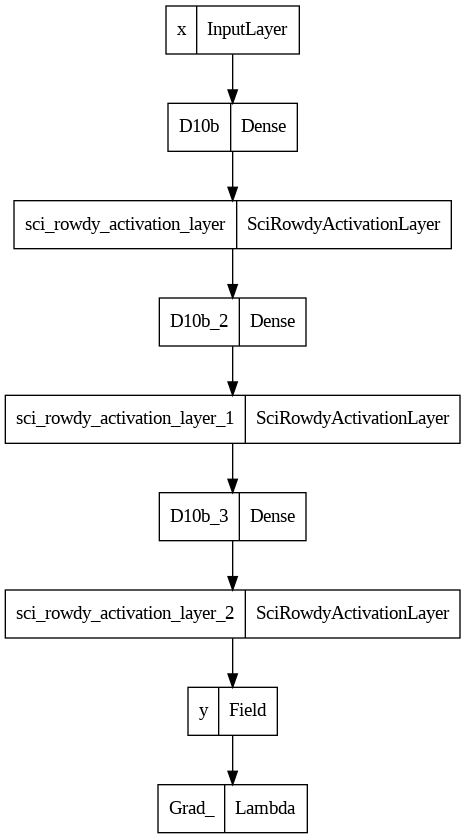
\includegraphics[width=0.5\textwidth]{img/sin.png}
    \caption{Esquema del modelo de \textit{SciANN} para la curva $y=sin(x)$.}
    \label{fig:sin}
\end{figure}


Cuando las restricciones vienen únicamente impuestas por datos el modelo mantiene una estructura secuencial, como puede verse en la \autoref{fig:sin}. 


\subsubsection{Resultados}

Uno de los objetivos de este experimento es medir cómo responden los predictores creados frente a distintos tamaños de conjunto de entrenamiento. Para ello, vamos a comenzar analizando los resultados obtenidos para un conjunto de entrenamiento con 10.000 elementos en el intervalo $[0,2\pi]$. Posteriormente, se realizará un análisis similar escogiendo 100 datos en el mismo intervalo. La sección finalizará haciendo una comparación de los resultados obtenidos. 

Para el conjunto de entrenamiento con 10.000 datos, tal y como se puede observar en la \autoref{fig:img73}, todos los modelos consiguen un error de predicción en el conjunto de entrenamiento cercano a cero, dando mejores resultados cuando los modelos no son demasiados simples. Estos resultados no se mantienen en validación. Aun así, comparando la \autoref{fig:img73} con la \autoref{fig:img74}, se puede observar una correspondencia entre los modelos que dan mejores resultados en \textit{loss} y los que los dan en \textit{val\_loss}. No es una correspondencia en magnitud, pero sí lo es a la hora de establecer una jerarquía entre los mejores modelos. 


\begin{figure}[htbp]
    \centering
    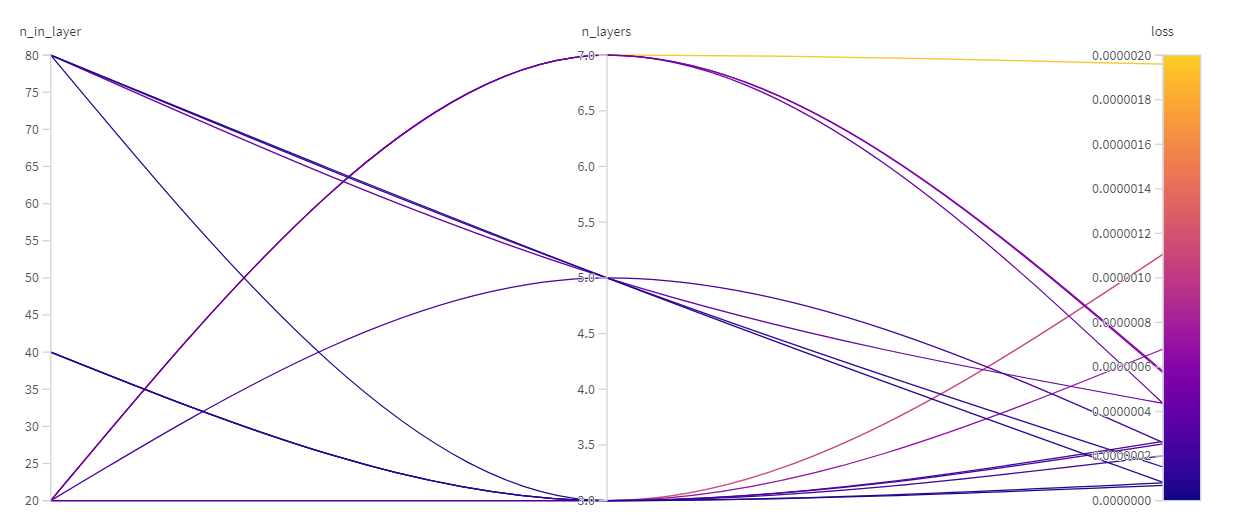
\includegraphics[width=1\textwidth]{img/img73.png}
    \caption{Desglose del ajuste de hiperparámetros para para la curva $y=sin(x)$ del experimento 8.1. con conjunto de entrenamiento ampliado bajo la métrica \textit{loss}.}
    \label{fig:img73}
\end{figure}

\begin{figure}[htbp]
    \centering
    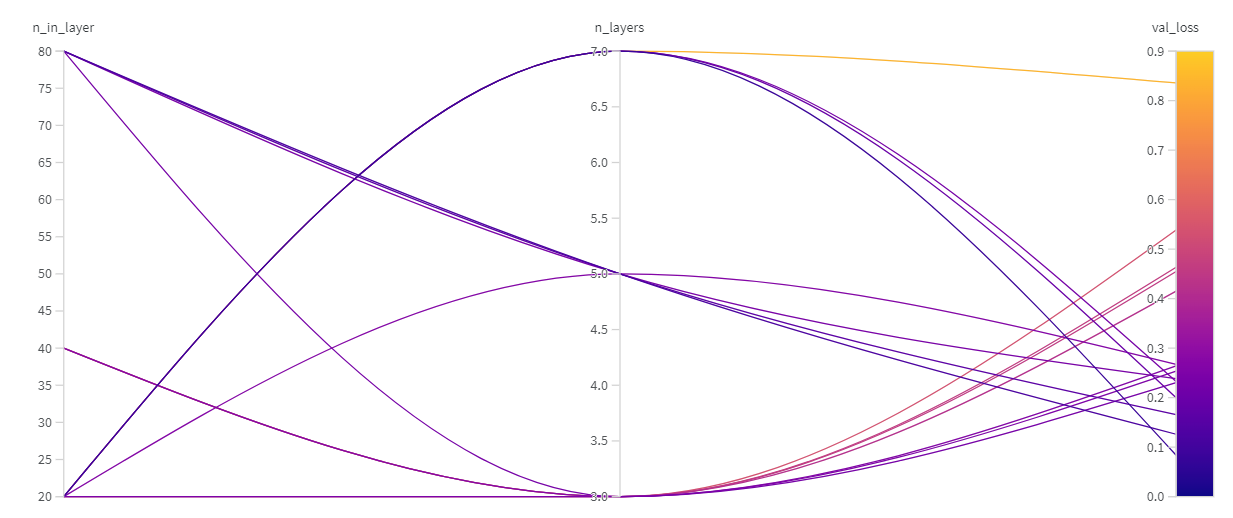
\includegraphics[width=1\textwidth]{img/img74.png}
    \caption{Desglose del ajuste de hiperparámetros para la curva $y=sin(x)$ del experimento 8.1. con conjunto de entrenamiento ampliado bajo la métrica \textit{val\_loss}.} 
    \label{fig:img74}
\end{figure}

Al hacer una representación gráfica de las predicciónes para el modelo con los hiperparámetros especificados en el \autoref{lst:exp1-sin}, podemos dar explicación a los resultados obtenidos. En la \autoref{fig:img07} se muestra el ajuste en entrenamiento mientras que en \autoref{fig:img08} se muestra la predicción para el conjunto de test. En ambos casos, se muestra en negro la función original y en rojo la predicción. Podemos ver cómo las gráficas originales se solapan con la predicción en el intervalo $[0,2\pi]$ y el error de validación viene, por tanto, de que el ajuste realizado es local: el modelo no es capaz de generalizar bien a datos de entrada fuera del intervalo para el que hemos aprendido a predecir. 



\begin{figure}[htbp]
    \centering
    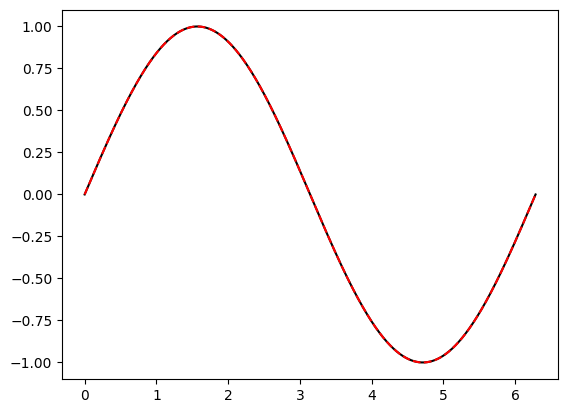
\includegraphics[width=0.5\textwidth]{img/img04.png}
    \caption{Ajuste de la curva $y=sin(x)$ en el intervalo $[0,2\pi ]$, donde la función original aparece en negro y la predicción en rojo.}
    \label{fig:img04}
\end{figure}

\begin{figure}[htbp]
    \centering
    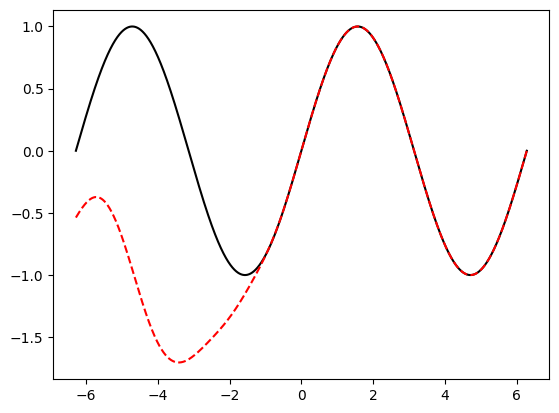
\includegraphics[width=0.5\textwidth]{img/img08.png}
    \caption{Predicción para la curva $y=sin(x)$ en el intervalo $[-2\pi,2\pi ]$, donde la función original aparece en negro y la predicción en rojo.}
    \label{fig:img08}
\end{figure}

El experimento continúa haciendo una búsqueda en el mismo espacio de parámetros, esta vez entrenando con un conjunto de 100 datos en la partición de $[0,2\pi]$. En la \autoref{fig:img77} podemos ver como las predicciones en entrenamiento han empeorado considerablemente. Al realizar una comparación con los resultados de validación, en la \autoref{fig:img76} vemos que, en contraste con los resultados en entrenamiento, el modelo generaliza igual de bien que el entrenado con más datos. Podríamos deducir, por tanto, que al dar al modelo tantos datos parecidos, creamos en el primer caso una situación de sobre-ajuste a dicho conjunto de entrenamiento. 

\begin{figure}[htbp]
    \centering
    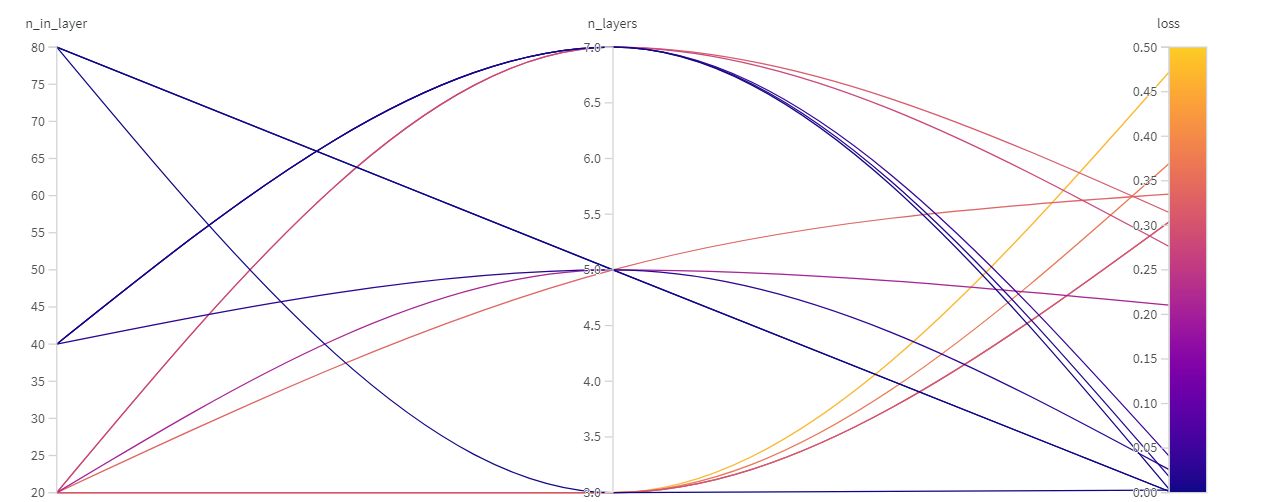
\includegraphics[width=1\textwidth]{img/img77.png}
    \caption{Desglose del ajuste de hiperparámetros para para la curva $y=sin(x)$ del experimento 8.1. con conjunto de entrenamiento reducido bajo la métrica \textit{loss}.}
    \label{fig:img77}
\end{figure}

\begin{figure}[htbp]
    \centering
    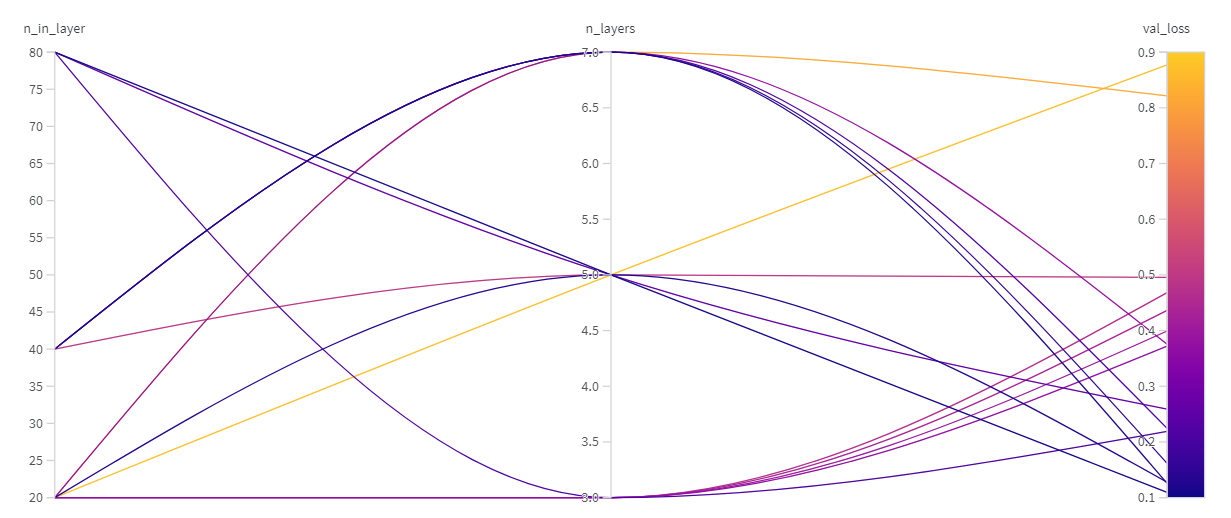
\includegraphics[width=1\textwidth]{img/img76.png}
    \caption{Desglose del ajuste de hiperparámetros para la curva $y=sin(x)$ del experimento 8.1. con conjunto de entrenamiento reducido bajo la métrica \textit{val\_loss}.} 
    \label{fig:img76}
\end{figure}

Continuamos realizando un estudio de la robustez de estos modelos frente a ruido. Para ello, se ha introducido ruido en el conjunto de entrenamiento de 10.000 datos. En la \autoref{fig:img71} y la \autoref{fig:img70} podemos apreciar que los valores de error en \textit{loss} y en \textit{val\_loss} son muy similares a los obtenidos para el entrenamiento sin ruido. Esto indica que el modelo ajusta igual de bien en ambos casos y corrobora que, en ambos modelos, el error en validación se debe al dominio de definición de la función para cada conjunto de entrenamiento. 

\begin{figure}[htbp]
    \centering
    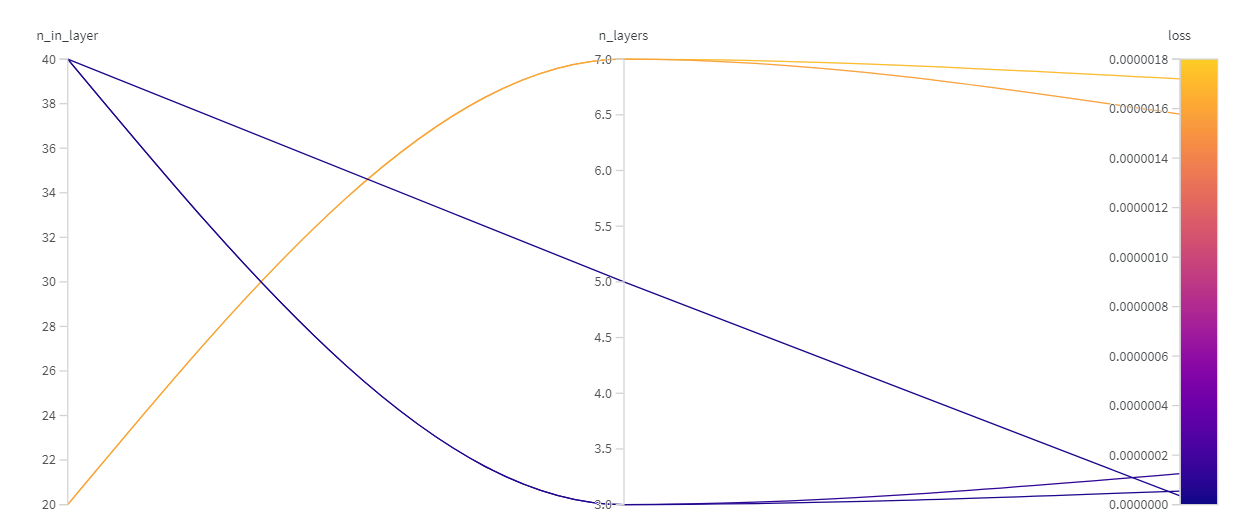
\includegraphics[width=1\textwidth]{img/img71.png}
    \caption{Desglose del ajuste de hiperparámetros para para la curva $y=sin(x)$ frente a ruido bajo la métrica \textit{loss}.}
    \label{fig:img71}
\end{figure}

\begin{figure}[htbp]
    \centering
    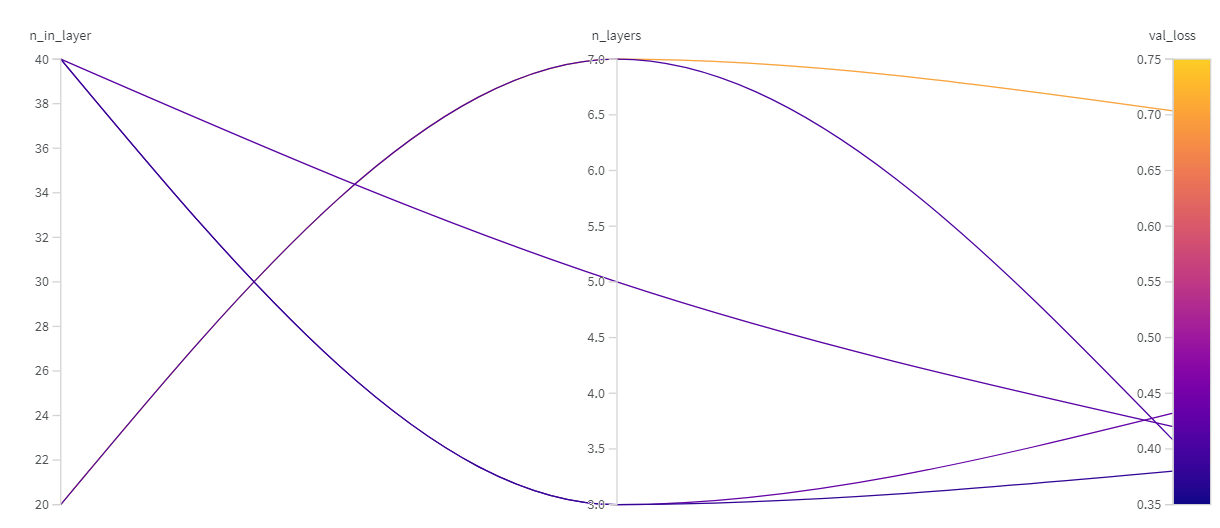
\includegraphics[width=1\textwidth]{img/img70.png}
    \caption{Desglose del ajuste de hiperparámetros para la curva $y=sin(x)$ frente a ruido. bajo la métrica \textit{val\_loss}.} 
    \label{fig:img70}
\end{figure}

Para evaluar cómo escalan los modelos vamos a realizar un estudio de las experimentaciones propuestas con respecto a su tiempo de ejecución. Los experimentos lanzados para el mayor conjunto de entrenamiento han tenido unos tiempos de ejecución en el rango de $[350,1050]$ segundos. Dentro de este rango, en la \autoref{fig:img45} podemos ver cómo el hiperparámetro más penalizado ha sido contar con un número de capas ocultas alto. Los resultados para la ejecución con ambosconjuntos de entrenamiento, mostrados en la \autoref{fig:img78} y la \autoref{fig:img75}, corroboran esta hipótesis. 

\begin{figure}[htbp]
    \centering
    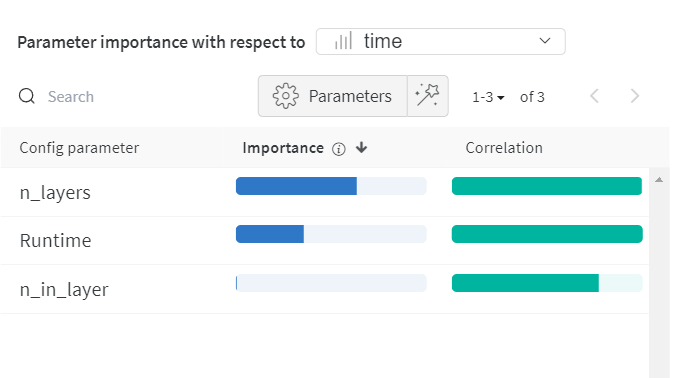
\includegraphics[width=0.5\textwidth]{img/img45.png}
    \caption{Ranking de parámetros correlacionados con la métrica \textit{time} para la curva $y=sin(x)$ del experimento 8.1.}
    \label{fig:img45}
\end{figure}


\begin{figure}[htbp]
    \centering
    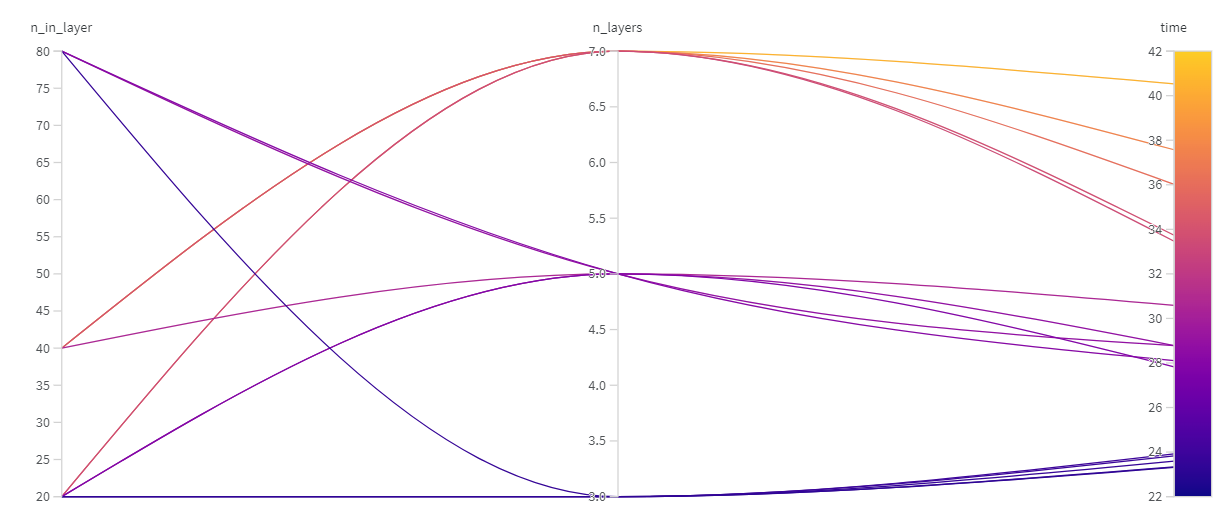
\includegraphics[width=1\textwidth]{img/img78.png}
    \caption{Desglose del ajuste de hiperparámetros para la curva $y=sin(x)$ del experimento 8.1. con conjunto de entrenamiento reducido bajo la métrica \textit{time}.}
    \label{fig:img78}
\end{figure}

\begin{figure}[htbp]
    \centering
    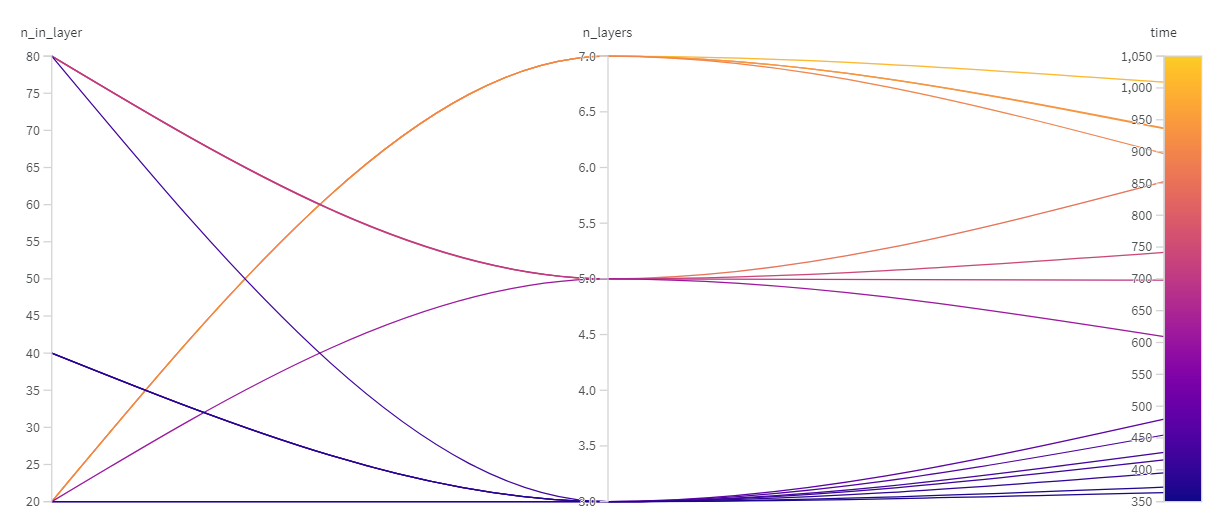
\includegraphics[width=1\textwidth]{img/img75.png}
    \caption{Desglose del ajuste de hiperparámetros para la curva $y=sin(x)$ del experimento 8.1. con conjunto de entrenamiento ampliado bajo la métrica \textit{time}.}
    \label{fig:img75}
\end{figure}


Por último, en la \autoref{fig:img27} mostramos un desglose de la evolución del error por cada término de la función de pérdida. Podemos observar que el modelo aprende más rápido de los datos propios de regresión que de los datos inferidos a través de la relación de diferenciación. 

\begin{figure}[htbp]
    \centering
    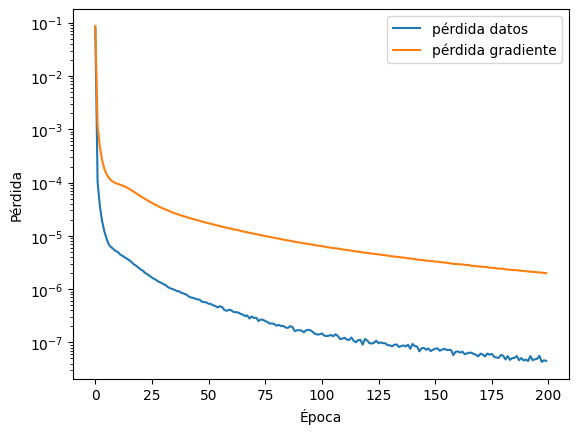
\includegraphics[width=0.6\textwidth]{img/img27.png}
    \caption{Evolución de los términos de la función de pérdida durante el entrenamiento para la curva $y=sin(x)$.}
    \label{fig:img27}
\end{figure}

Con todo esto, podemos concluir que \textit{SciANN} es capaz de completar satisfactoriamente tareas sencillas de regresión dentro del intervalo de definición estipulado en el entrenamiento. Además, estas tareas son sensibles tanto al número de capas profundas del modelo seleccionado como al tamaño del conjunto de entrenamiento. 

\subsection{Ajuste de la función exponencial}
Este segundo experimento pretende reflejar la capacidad de \textit{SciANN} para ajustar funciones en un caso para el que no disponemos de tanta información sobre los parámetros óptimos para el aprendizaje. Puesto que el objetivo es el mismo que en el experimento anterior, la estructura del modelo de \textit{SciANN} se conserva, como puede observarse en el \autoref{lst:exp1-exp}. 

Como desconocemos la complejidad del modelo necesario para hacer un buen ajuste, se ha experimentado con la densidad de la red neuronal asociada a la función exponencial, así como con sus funciones de activación. Además de esto, se ha hecho un ajuste de los hiperparámetros más relevantes de toda tarea de entrenamiento en aprendizaje profundo: la tasa de aprendizaje y el tamaño de lote. Con respecto a la evolución del entrenamiento, se ha optado por utilizar el procedimiento de parada anticipada para garantizar un número de épocas adecuado.

%En cuanto a las funciones de activación, nos decantamos por utilizar ReLU debido a su buen rendimiento en general. Como el resultado del experimento fue lo suficiéntemente bueno, no fue necesaria la búsqueda de funciones de activación más específicas para el problema. Con respecto a la programación del ritmo de aprendizaje, volvimos a escoger decaimiento exponencial ya que, de nuevo, suele funcionar bien y por tanto es un buen candidato inicial. Para asegurar un aprendizaje correcto y prevenir una situación de sobreajuste, fijamos un número de épocas elevado e intervenimos en el entrenamiento mediante la técnica de regularización de parada anticipada.


\definecolor{codegreen}{rgb}{0,0.6,0}
\definecolor{codegray}{rgb}{0.5,0.5,0.5}
\definecolor{codepurple}{rgb}{0.58,0,0.82}
\definecolor{backcolour}{rgb}{0.95,0.95,0.92}

\lstdefinestyle{mystyle}{
    backgroundcolor=\color{backcolour},   
    commentstyle=\color{codegreen},
    keywordstyle=\color{magenta},
    numberstyle=\tiny\color{codegray},
    stringstyle=\color{codepurple},
    basicstyle=\ttfamily\footnotesize,
    breakatwhitespace=false,         
    breaklines=true,                 
    captionpos=b,                    
    keepspaces=true,                 
    numbers=left,                    
    numbersep=5pt,                  
    showspaces=false,                
    showstringspaces=false,
    showtabs=false,                  
    tabsize=2
}

\lstset{style=mystyle}


\begin{lstlisting}[language=Python,caption={Ejemplo de modelo en \textit{SciANN} para el ajuste de la función exponencial.},label={lst:exp1-exp}]
#Definimos la estructura de la función que queremos aprender.
x = Variable('x')
y = Functional('y', x, 5*[20], activation=5*['tanh'])

#Imponemos restricciones al modelo.
dy_dx = sn.diff(y, x)
c1 = Data(y)

#Definimos el modelo.
model = SciModel(x, [y, dy_dx], optimizer='adam')

start_time = time.time()

#Entrenamiento.
entrenamiento_exp = model.train(x_true,
            [y_true, dy_true],
            epochs=10000,
            learning_rate=0.01,
            batch_size=128,
            callbacks=[keras.callbacks.EarlyStopping(monitor="loss",
                        min_delta = 0, patience=20,verbose=1)]
            )
\end{lstlisting}

%\begin{figure}[htbp]
 %   \centering
 %   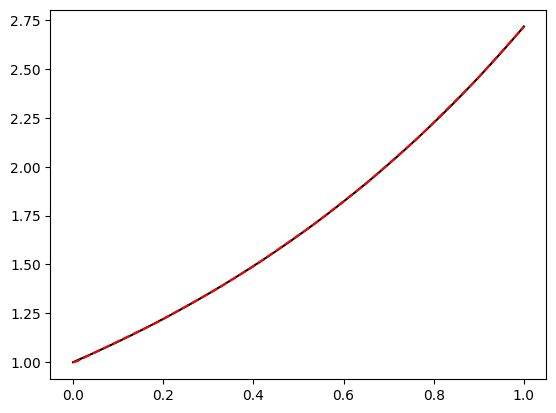
\includegraphics[width=0.5\textwidth]{img/img05.png}
 %   \caption{Ajuste de la curva $y=exp(x)$ en el intervalo $[0,1 ]$.}
 %   \label{fig:img05}
%\end{figure}


\subsubsection{Resultados}

En la \autoref{fig:img79} podemos observar cómo el modelo que minimiza la pérdida en validación cuenta con cinco capas ocultas con $20$ neuronas y activación de tangente hiperbólica. En general, la experimentación refleja cómo modelos más complejos (con muchas capas ocultas o muchas neuronas por capa) son más propensos a responder mal ante la tarea. Además, el ranking proporcionado por \textit{W\&B} de la \autoref{fig:img84} muestra que el único hiperparámetro que parece estar correlacionado con menores valores de función de pérdida es la función de activación sigmoidal. En la \autoref{fig:img82} podemos ver cómo el modelo seleccionado en validación también es uno de los que mejor se ajusta al conjunto de entrenamiento. 


\begin{figure}[htbp]
    \centering
    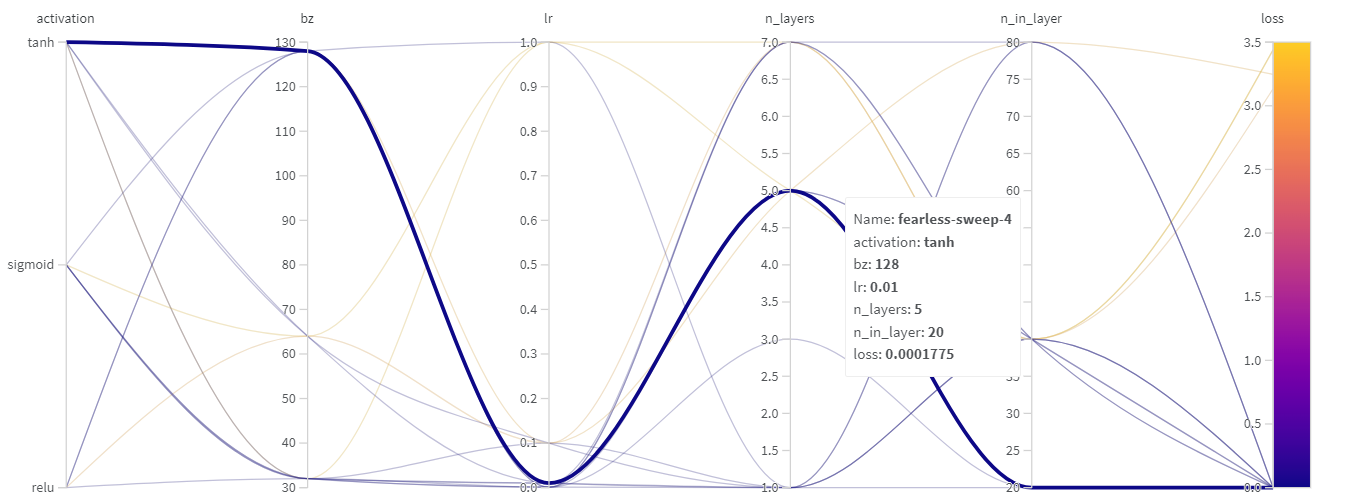
\includegraphics[width=1\textwidth]{img/img82.png}
    \caption{Desglose del ajuste de hiperparámetros para para la curva $y=exp(x)$ del experimento 8.1. bajo la métrica \textit{loss}.}
    \label{fig:img82}
\end{figure}

\begin{figure}[htbp]
    \centering
    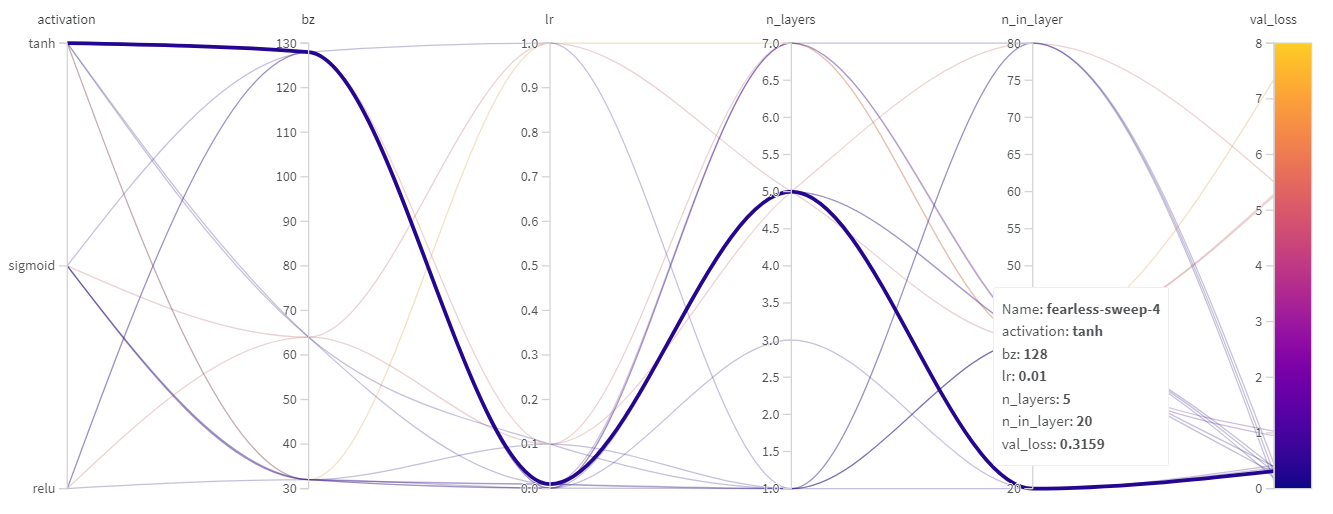
\includegraphics[width=1\textwidth]{img/img79.png}
    \caption{Desglose del ajuste de hiperparámetros para la curva $y=exp(x)$ del experimento 8.1.  bajo la métrica \textit{val\_loss}.} 
    \label{fig:img79}
\end{figure}

\begin{figure}[htbp]
    \centering
    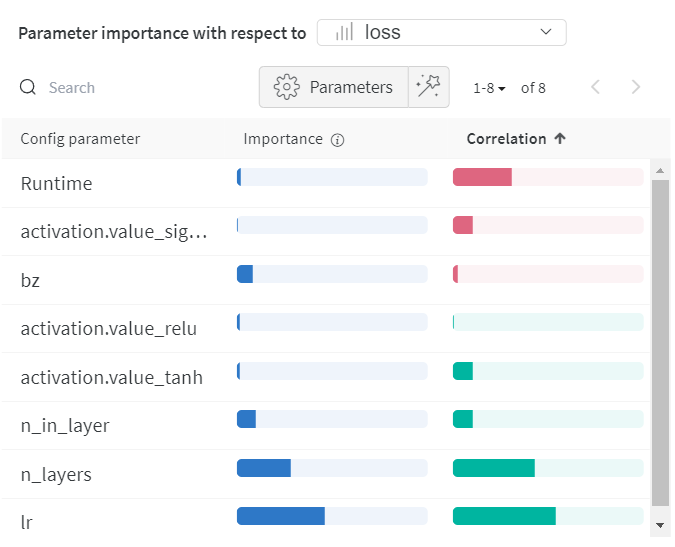
\includegraphics[width=0.5\textwidth]{img/img84.png}
    \caption{Ranking de parámetros correlacionados con la métrica \textit{loss} para la curva $y=exp(x)$ del experimento 8.1.}
    \label{fig:img84}
\end{figure}

En cuanto a los tiempos de ejecución del entrenamiento, en la \autoref{fig:img81} podemos ver que quedan dentro del intervalo de $[7,100]$ segundos. A simple vista es difícil encontrar una correlación directa entre alguno de los hiperparámetros y el tiempo de entrenamiento, pero a través del ranking proporcionado por \textit{W\&B}, que se muestra en la \autoref{fig:img83}, se ha detectado que la función de activación sigmoidal está correlacionada con mayores tiempos de entrenamiento. Sin embargo, una visualización más clara de la correlación entre las funciones de activación y la métrica \textit{time}, que se muestra en la \autoref{fig:img85}, deja ver que la relación encontrada se debe a que, en la búsqueda aleatoria de configuraciones, se han dado varias configuraciones en las que la función sigmoidal iba asociada a tasas de aprendizaje muy pequeñas junto con modelos complejos, con muchas capas densas. Es por esto que el ranking nos da esa 
información. 

\begin{figure}[htbp]
    \centering
    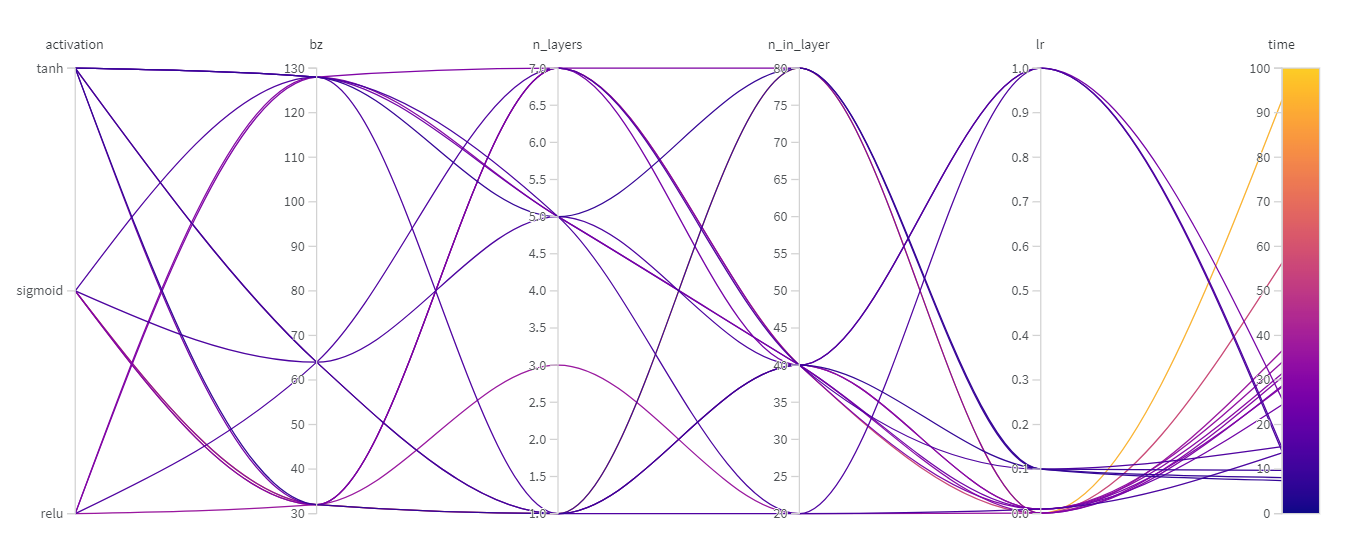
\includegraphics[width=1\textwidth]{img/img81.png}
    \caption{Desglose del ajuste de hiperparámetros para la curva $y=exp(x)$ del experimento 8.1.  bajo la métrica \textit{time}.}
    \label{fig:img81}
\end{figure}


\begin{figure}[htbp]
    \centering
    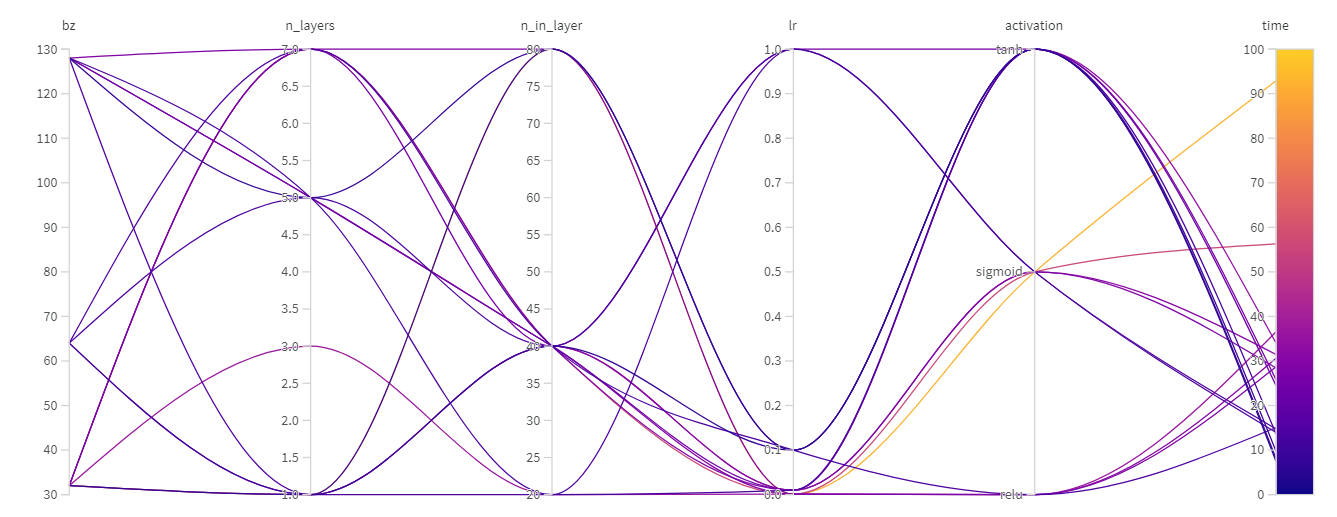
\includegraphics[width=1\textwidth]{img/img85.png}
    \caption{Segundo desglose del ajuste de hiperparámetros para la curva $y=exp(x)$ del experimento 8.1.  bajo la métrica \textit{time}.}
    \label{fig:img85}
\end{figure}

\begin{figure}[htbp]
    \centering
    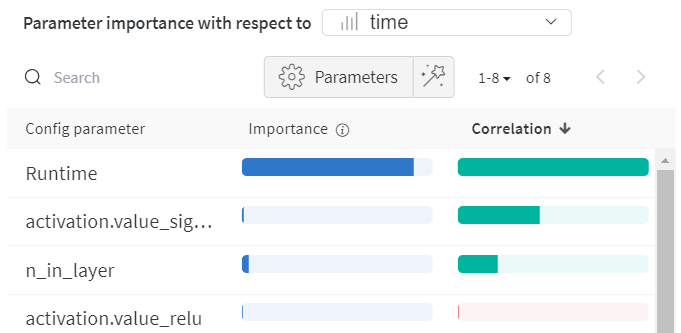
\includegraphics[width=0.5\textwidth]{img/img83.png}
    \caption{Ranking de parámetros correlacionados con la métrica \textit{time} para la curva $y=exp(x)$ del experimento 8.1.}
    \label{fig:img83}
\end{figure}


Procedemos por tanto a realizar un análisis más detallado de la evolución del entrenamiento para el modelo que ha minimizado la pérdida en validación. De manera análoga al experimento anterior, en la \autoref{fig:img86} podemos ver cómo la predicción es buena únicamente dentro del intervalo de entrenamiento. Sin embargo, en contraposición con el mismo, la \autoref{fig:img87} muestra que en este caso el entrenamiento se ha beneficiado por igual de la pérdida inducida por los datos de la función que de la inducida por los datos del gradiente. 

\begin{figure}[htbp]
    \centering
    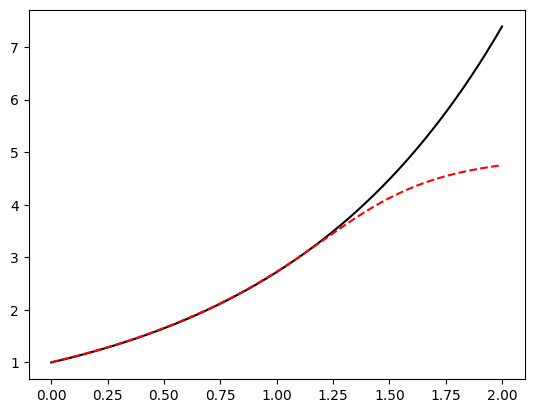
\includegraphics[width=0.5\textwidth]{img/img86.png}
    \caption{Predicción para la curva $y=exp(x)$ en el conjunto de validación, donde dibujamos en negro el valor real de la función y en rojo la predicción.}
    \label{fig:img86}
\end{figure}

\begin{figure}[htbp]
    \centering
    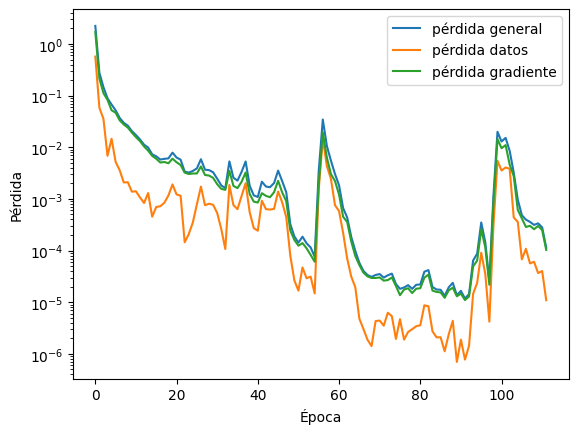
\includegraphics[width=0.6\textwidth]{img/img87.png}
    \caption{Evolución de los términos de la función de pérdida durante el entrenamiento del modelo espeficiado en el \autoref{lst:exp1-exp} para la curva $y=exp(x)$.}
    \label{fig:img87}
\end{figure}


\subsection{Ajuste bidimensional}

\subsubsection{Generación de datos sintéticos}
Para este problema se ha creado un mallado en Numpy con una granularidad de $100\times 100$ datos. En la figura \autoref{fig:img06} se muestra la función evaluada en el dominio $[0,\pi]\times [0,\pi]$.
 \begin{figure}[htbp]
    \centering
    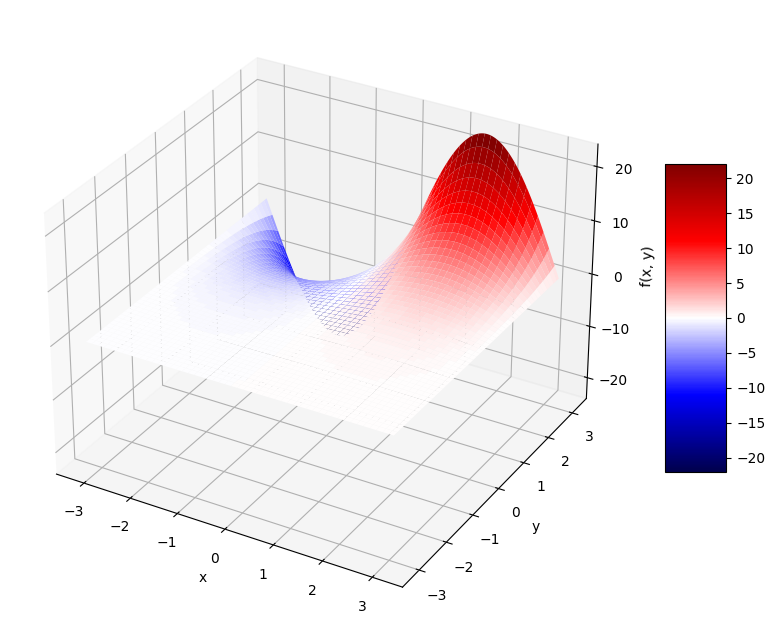
\includegraphics[width=0.5\textwidth]{img/img06.png}
    \caption{Ajuste de la curva $z=\sin(x)e^{y}$ en el intervalo $[0,\pi]\times [0,\pi]$.}
    \label{fig:img06}
\end{figure}

\subsubsection{Construcción del modelo}

El modelo, que queda detallado en el \autoref{lst:exp1-bidim}, es similar a los descritos anteriormente. Como tenemos dos variables de entrada, ambas unidimensionales, hemos definido un total de dos objetos \textit{Variable} para el modelo. Además, al tratarse de un problema algo más complejo, hemos aumentado el número de capas densas. 

\begin{lstlisting}[language=Python,caption={Modelo en \textit{SciANN} para ajuste bidimensional.},label={lst:exp1-bidim}]
    #Definición de las entradas.
    x = sn.Variable('x')
    y = sn.Variable('y')
    
    #Definición de la función.
    f = sn.Functional('f', [x, y], [10, 10, 10, 10], 'tanh')
    
    #Imposición de restricciones.
    df_dx = sn.diff(f, x)
    df_dy = sn.diff(f, y)
    
    d1 = sn.Data(f)

    #Definición del modelo.
    modelo_2d = sn.SciModel([x,y],[f, df_dx,df_dy])
\end{lstlisting}

En la \autoref{fig:2D} podemos ver cómo se mantiene la estructura secuencial debido a que, una vez más, únicamente hemos impuesto restricciones que vengan únicamente a partir de datos explícitos. 

 \begin{figure}[htbp]
    \centering
    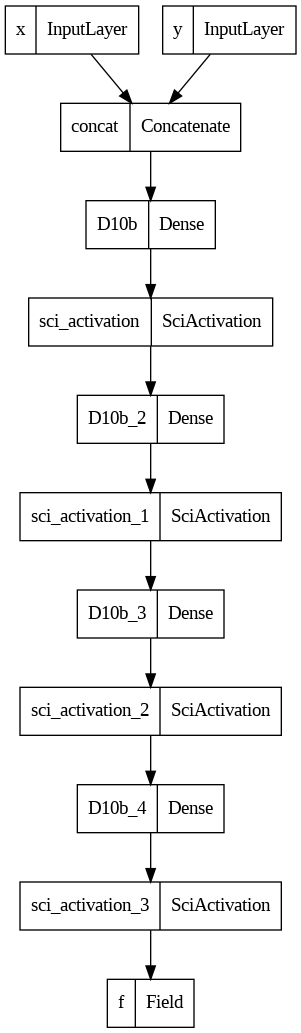
\includegraphics[width=0.3\textwidth]{img/2D.png}
    \caption{Esquema de red neuronal para la curva $z=\sin(x)e^{y}$.}
    \label{fig:2D}
\end{figure}

\subsubsection{Resultados}

Como podemos ver en la \autoref{fig:img07}, la aproximación solo es buena localmente, en el dominio de entrenamiento. En la evolución del entrenamiento (recogida en \autoref{fig:img28}) se puede observar como, al igual que en el primer experimento, el aprendizaje viene sobre todo de los datos explícitos de la función. En cuanto al tiempo de entrenamiento, la media ha sido de $532,631$ segundos.
\begin{figure}[htbp]
    \centering
    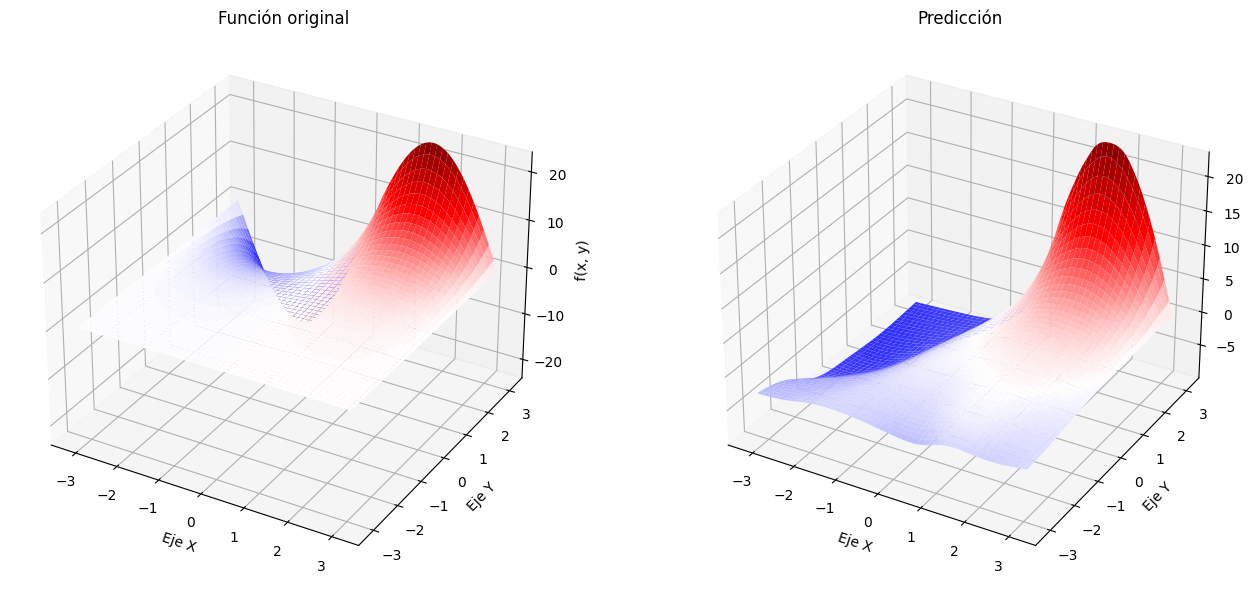
\includegraphics[width=0.7\textwidth]{img/img07.png}
    \caption{Comparación de la función original con la predicción de \textit{SciANN}.}
    \label{fig:img07}
\end{figure}
\begin{figure}[htbp]
    \centering
    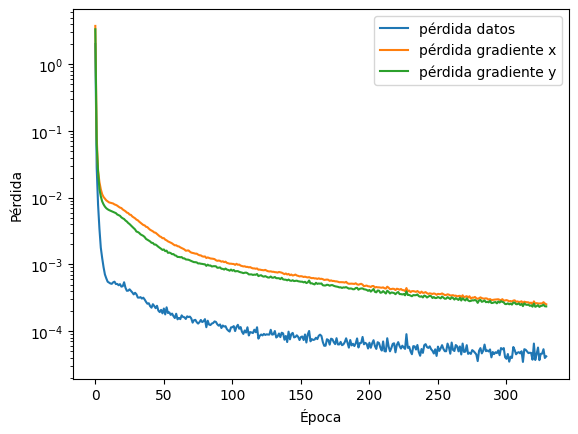
\includegraphics[width=0.5\textwidth]{img/img28.png}
    \caption{Evolución de los términos de la función de pérdida durante el entrenamiento para la curva $z=\sin(x)e^{y}$.}
    \label{fig:img28}
\end{figure}



\section{Experimento 2: El problema de Burgers}

Este experimento tiene como objetivos exponer los conocimientos adquiridos en referencia al modelado de PINNs y estudiar cómo afecta la complejidad del modelo a la eficiencia de la tarea de aprendizaje en \textit{SciANN}. 

\subsection{Descripción del problema}

El problema de Burgers describe los fenómenos de advección y difusión que modelan, entre otros, la evolución de la velocidad en un fluido o la densidad del tráfico. Se utiliza ampliamente en la dinámica de fluidos y la teoría del tráfico. En 2018 se abrió la puerta a su modelado mediante el uso de redes neuronales profundas~\cite{Raissi2018}. El modelo se rige por la ecuación:
\begin{equation}
\frac{\partial u}{\partial t} + u \frac{\partial u}{\partial x} = \nu \frac{\partial^2 u}{\partial x^2}
\end{equation}

donde $\nu$ es un parámetro que representa la viscosidad cinemática y $u(t,x)$ representa la velocidad. El término de advección $u \frac{\partial u}{\partial x}$  describe el transporte de una sustancia o propiedad (como el calor o la humedad) a través de un fluido en movimiento e introduce no-linealidad en este problema. Representa cómo la velocidad del fluido en un punto afecta al cambio de velocidad en el espacio. Reproduciendo el experimento descrito en~\cite{Raissi2018}, vamos a trabajar con una versión unidimensional del problema 
$$
\frac{\partial u}{\partial t} + u \frac{\partial u}{\partial x} = (\frac{0.01}{\pi}) \frac{\partial^2 u}{\partial x^2}, \quad t \in [0, 1],\quad x \in [-1,1]
$$
sujeta a las condiciones iniciales y de contorno
$$
u(0, x) = -\sin(\pi x), \quad u(t, 1) = 0, \quad u(t, -1) = 0.
$$
\subsection{Generación de datos sintéticos}

Siguiendo la estructura de entrada que \textit{SciANN} requiere, es necesario construir un mallado del espacio de entrada $[0,1]\times[-1,1]$. Como los objetivos del entrenamiento no son ajustarnos a unos valores de salida, si no cumplir con una serie de restricciones, en este experimento no generaremos datos explícitos de salida para $u(t,x)$. 

\subsection{Construcción del modelo}
Nuestro objetivo es, por tanto, construir un aproximador 
$\hat{u}(t, x)$ de $u(t,x)$ definido en el dominio $[0,1]\times[-1,1]$.
\begin{lstlisting}[language=Python,caption={Modelo en \textit{SciANN} para el problema de Burgers.},label={lst:exp2}]
#Definición de entradas.
x = sn.Variable('x')
t = sn.Variable('t')

#Definicón de la función a aprender.
u = sn.Functional('u', [t,x], 8*[20], 'tanh')

#Definición de las restricciones del modelo. 
L1 = diff(u, t) + u*diff(u,x) - (0.01/pi)*diff(u, x, order=2)
TOL = 0.001
C1 = (1-sign(t - TOL)) * (u + sin(pi*x))
C2 = (1-sign(x - (-1+TOL))) * (u)
C3 = (1+sign(x - ( 1-TOL))) * (u)

#Definición del modelo.
burgers_model = sn.SciModel([x, t], [L1, C1, C2, C3])
\end{lstlisting}

Como podemos observar en el \autoref{lst:exp2}, los elementos principales utilizados para la construcción de $\hat{u}(t,x)$ son:

\begin{itemize}

    \item Variables de entrada: Definimos un objeto `t' de tipo \textit{Variable} para la variable temporal y un único objeto `x' de tipo \textit{Variable} para la variable espacial unidimensional.
    
    \item Funciones: Nuestro objetivo es aprender una única función, por lo que definimos un único objeto \textit{Functional}. Como esta tarea de aprendizaje es considerablemente más compleja que las anteriores, contamos con un mayor número de capas. Además, hemos seleccionado la tangente hiperbólica como función de activación ya que tiene una media más cercana a $0$ que otras funciones de activación, lo que permite preservar la varianza entre las entradas y salidas de cada capa y, por tanto, ayuda a la tarea de aprendizaje haciendo que los gradientes no se aproximen demasiado a $0$ en las capas internas. 
    
    \item Restricciones: Definimos tanto el PDE asociado (L1) como las condiciones iniciales y de contorno especificadas (C1,C2,C3). En vez de imponer de forma estricta estas condiciones, damos un margen de tolerancia de $0.001$. Esta decisión ha sido tomada con el propósito de facilitar la tarea de aprendizaje y acelerar así la convergencia del modelo. 
\end{itemize}

Observemos como, en contraposición con el experimento anterior, el objetivo del modelo es únicamente aproximar, es decir, no es necesario proporcionar de forma explícita evaluaciones discretas de $u(t,x)$: el cumplimiento de las restricciones definidas para cada entrada $(t,x)$ nos permitirá predecir la función $u(t,x)$. Esta configuración induce una estructura no secuencial en el modelo, como muestra la \autoref{fig:burgers}.

\begin{figure}[htbp]
    \centering
    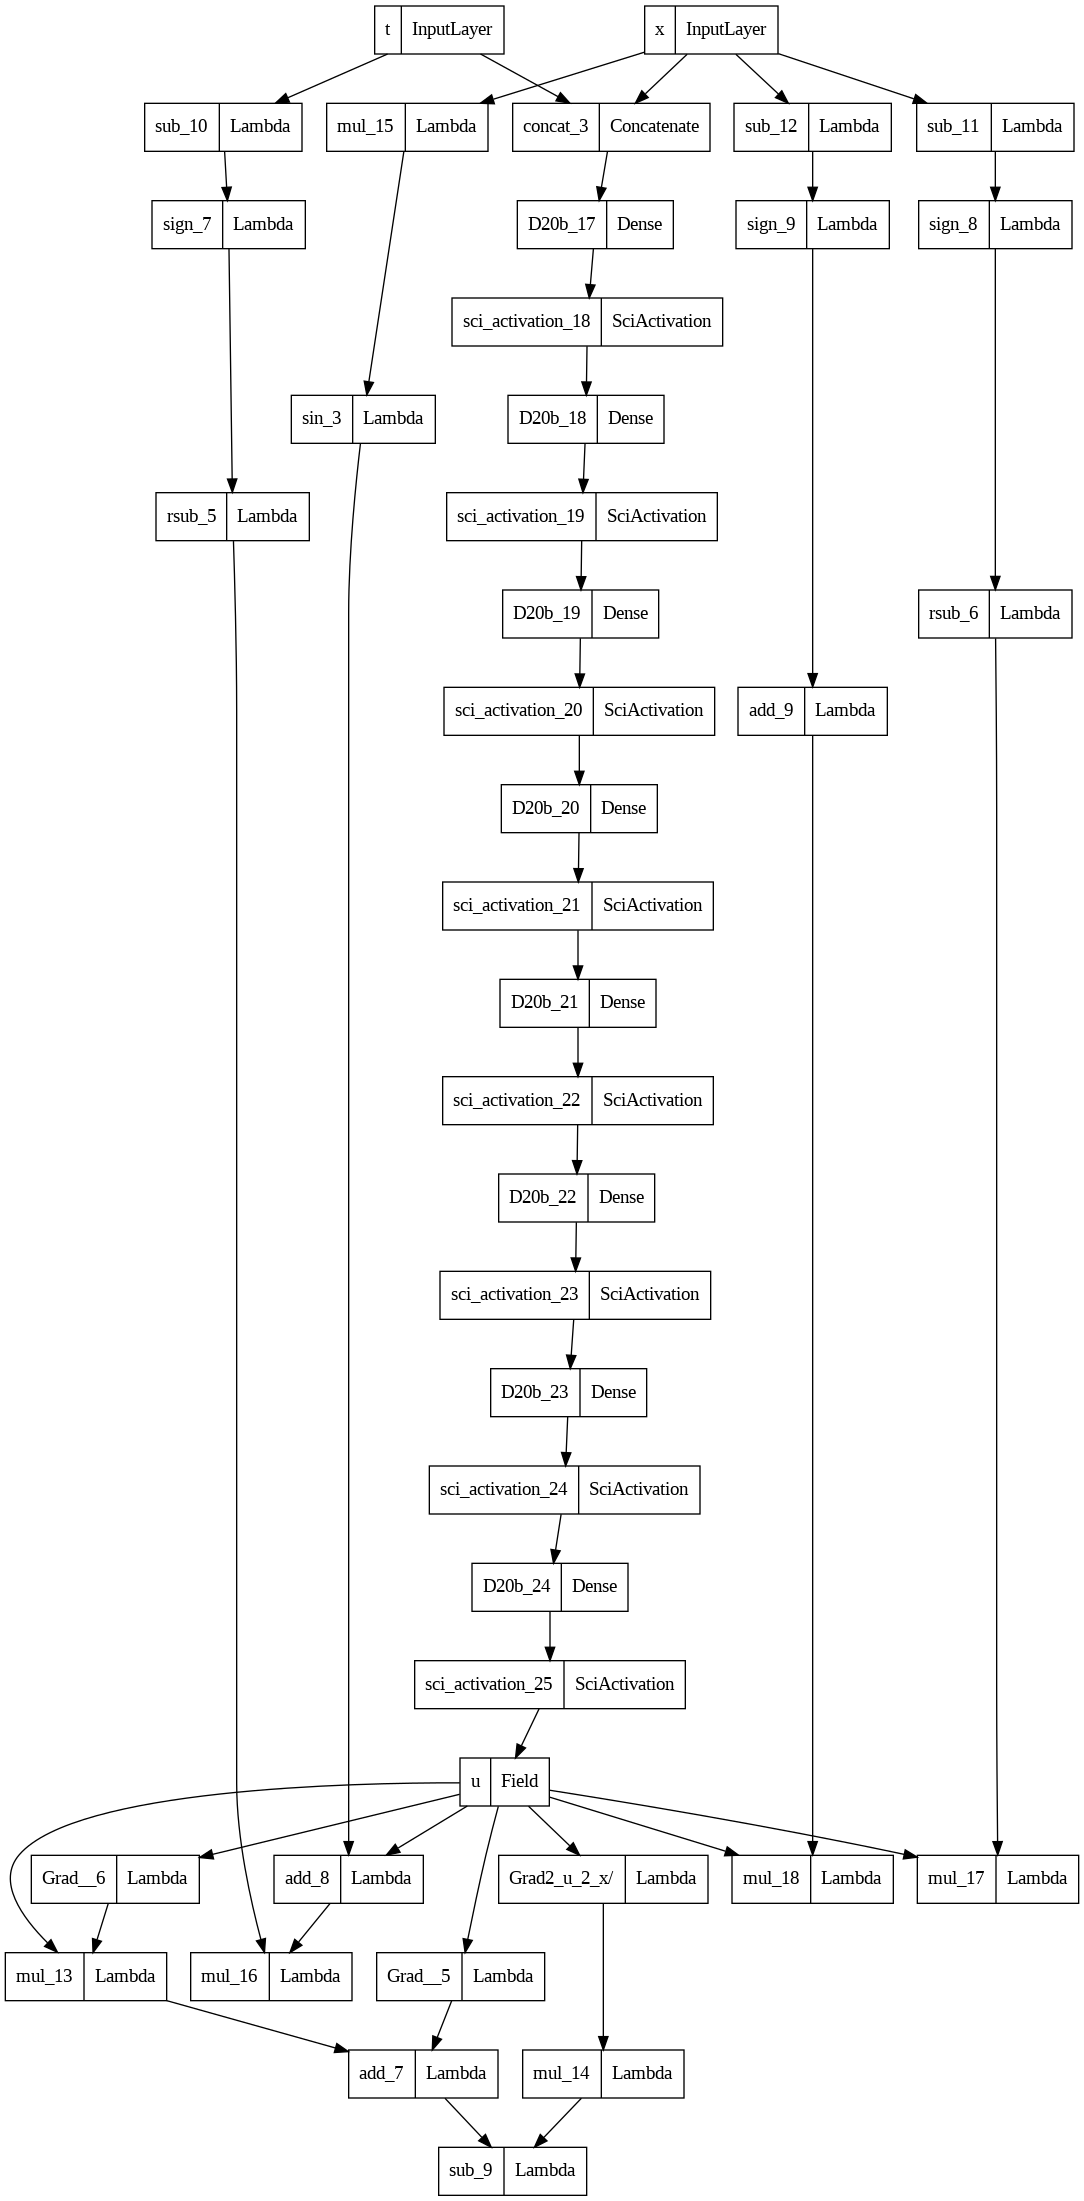
\includegraphics[width=0.66\textwidth]{img/burgers.png}
    \caption{Representación interna en \textit{SciANN} para el problema de Burgers.}
    \label{fig:burgers}
\end{figure}


\subsection{Resultados}

Los resultados obtenidos tras la experimentación (la \autoref{fig:img52} muestra los valores de pérdida y la \autoref{fig:img53} muestra los tiempos de entrenamiento) son bastante uniformes y no arrojan mucha luz. Además, se puede observar que el ajuste no es demasiado bueno, habiéndose encontrado otras implementaciones en~\cite{Haghighat2021} que han dado resultados con pérdidas del orden de $10^{-6}$. Tras una experimentación manual y visualizar la función de pérdida para el modelo descrito en el \autoref{lst:exp2}, en la \autoref{fig:img09} podemos observar cómo el aprendizaje es bastante errático, lo que hace que el método de parada anticipada no haya funcionado bien en nuestra experimentación. 



\begin{figure}[htbp]
    \centering
    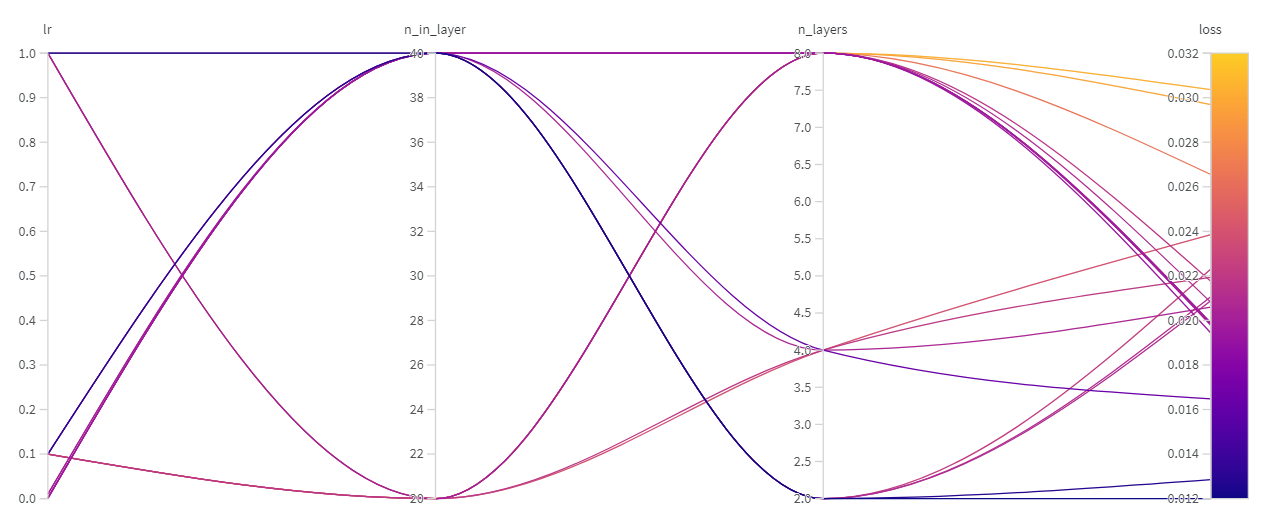
\includegraphics[width=1\textwidth]{img/img52.png}
    \caption{Desglose del ajuste de hiperparámetros para el problema de Burgers con parada anticipada bajo la métrica \textit{loss}.}
    \label{fig:img52}
\end{figure}

\begin{figure}[htbp]
    \centering
    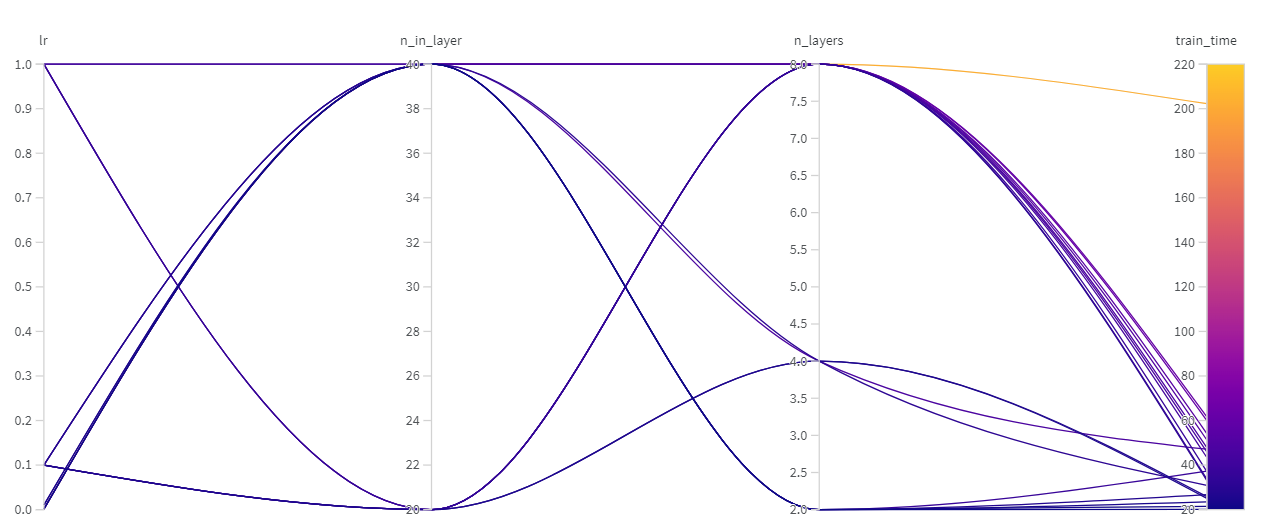
\includegraphics[width=1\textwidth]{img/img53.png}
    \caption{Desglose del ajuste de hiperparámetros para el problema de Burgers con parada anticipada bajo la métrica \textit{train\_time}.}
    \label{fig:img53}
\end{figure}


Procedemos, por tanto, a repetir la experimentación para un número de épocas fijo lo suficiéntemente grande. Los resultados mostrados en la \autoref{fig:img58} y la \autoref{fig:img59} corresponden al entrenamiento con un mallado de $1000$ datos y $3000$ épocas completas. Como podemos ver, una vez más, el hiperparámetro más importante en términos de eficiencia vuelve a ser el número de capas ocultas. Además, en la  \autoref{fig:img59} se aprecia que el ajuste es mejor para modelos más simples. 

\begin{figure}[htbp]
    \centering
    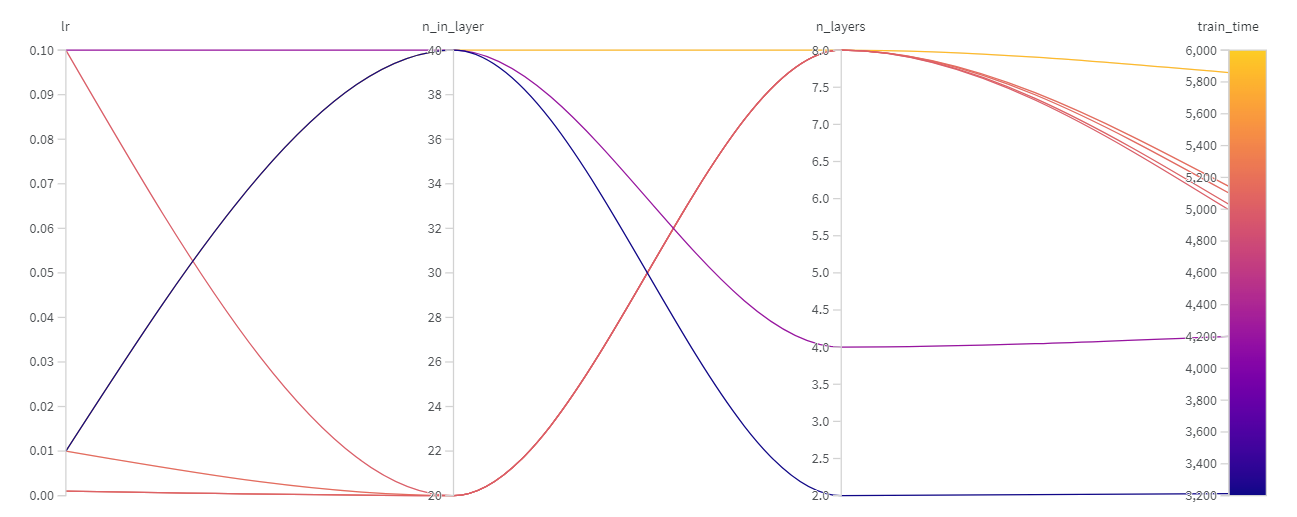
\includegraphics[width=1\textwidth]{img/img58.png}
    \caption{Desglose del ajuste de hiperparámetros para el problema de Burgers sin parada anticipada bajo la métrica \textit{train\_time}.}
    \label{fig:img58}
\end{figure}

\begin{figure}[htbp]
    \centering
    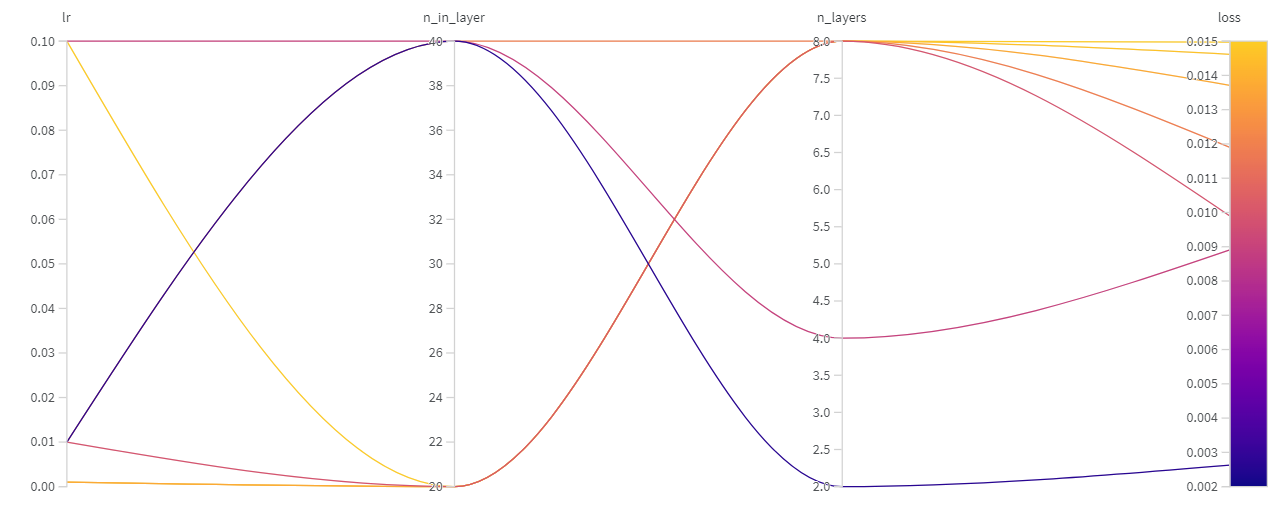
\includegraphics[width=1\textwidth]{img/img59.png}
    \caption{Desglose del ajuste de hiperparámetros para el problema de Burgers sin parada anticipada bajo la métrica \textit{loss}.}
    \label{fig:img59}
\end{figure}

A la vista de los resultados obtenidos, sigue siendo difícil justificar hasta qué punto estos tiempos de ejecución se deben a la complejidad del modelo o a la naturaleza del problema. Por ello, se ha realizado un estudio comparativo de los modelos seleccionados en el \autoref{lst:exp1-sin} y \autoref{lst:exp2}, por ofrecer valores de pérdida equivalentes en sus respectivas tareas de aprendizaje. Lo primero que nos llama la atención tras una comparación directa entre el tiempo de ejecución por época señala que cada época del  \autoref{lst:exp2} triplica los tiempos del \autoref{lst:exp1-sin}.  Como vimos en la \autoref{sec:8.2}, el entrenamiento en \textit{SciANN} es muy sensible al tamaño de conjunto de datos. Sin embargo, este factor no es influyente en nuestro problema ya que el experimento asociado al \autoref{lst:exp1-sin} iba asociado a un conjunto de entrenamiento mayor que el seleccionado para el problema de Burgers. 

Por otro lado, se ha explorado el resumen de ambos modelos. Para las implementaciones propuestas, \autoref{lst:exp1-sin} y \autoref{lst:exp2} tienen $233$ y $3021$ parámetros respectivamente. Por tanto, la variación de tiempos por época recae exclusivamente en la complejidad del modelo. 

\begin{figure}[htbp]
    \centering
    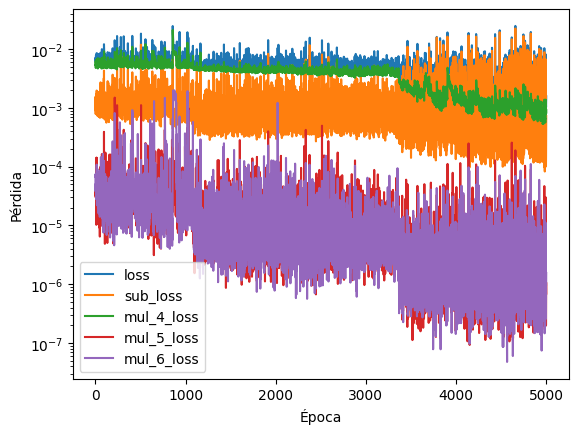
\includegraphics[width=0.5\textwidth]{img/img30.png}
    \caption{Evolución de la función de pérdida en el experimento 2.}
    \label{fig:img09}
\end{figure}


Por último, en la \autoref{fig:img1029} podemos comparar la predicción obtenida para el modelo de \autoref{lst:exp2} con los valores reales de $u$. Podemos por tanto concluir que, aunque la predicción es buena, la tarea de aprendizaje es muy poco directa, como quedó reflejado en la \autoref{fig:img09}. Esto hace que necesitemos una tarea de aprendizaje muy larga, lo que conlleva un coste computacional muy elevado. Sería necesario un estudio posterior para determinar hasta qué punto este coste computacional se debe a la implementación de \textit{SciANN} o a la complejidad del modelo en si. 

\begin{figure}[htbp]
    \centering
    \begin{subfigure}{0.3\textwidth}
    \centering
    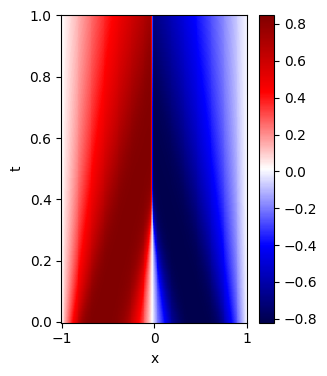
\includegraphics[width=\linewidth]{img/img10.png} 
    \caption{Predicción $\hat{u}$.}
    \label{fig:img10}
    \end{subfigure}   
    \begin{subfigure}{0.3\textwidth}
    \centering
    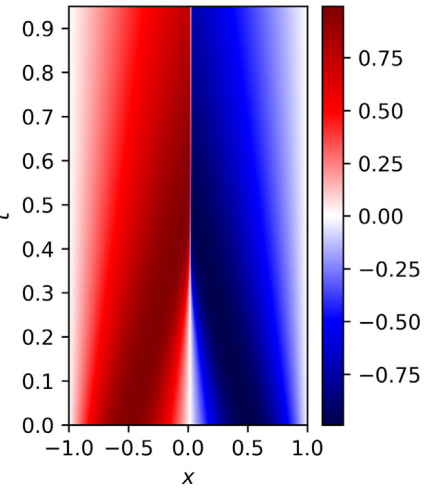
\includegraphics[width=\linewidth]{img/img29.png}
    \caption{Evaluación real de $u$.}
    \label{fig:img29}
    \end{subfigure}
    \begin{subfigure}{0.235\textwidth}
    \centering
    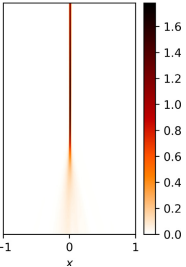
\includegraphics[width=\linewidth]{img/img88.png}
    \caption{$\vert u- \hat{u}\vert$.}
    \label{fig:img88}
    \end{subfigure}
\caption{Comparación de $\hat{u}$ y $u$  en el problema de Burgers extraída de~\cite{Haghighat2021}.}
\label{fig:img1029}
\end{figure}



\section{Experimento 3: Aproximación de operadores}
\subsection{Motivación}


Hasta ahora se ha mostrado la capacidad de \textit{SciANN} para aproximar funciones partiendo de información explícita o implícita sobre ellas. Con este experimento se pretende poner a prueba la capacidad de \textit{SciANN} para aproximar operadores bajo la hipótesis de que, como vimos en el~\autoref{ch:sexto-capitulo}, tomando un número lo suficiéntemente grande de neuronas por capa, es posible alcanzar una buena aproximación, sea cual sea nuestra elección de función de activación para el modelo. El experimento tiene otro objetivo que es la comparación de \textit{SciANN} con \textit{DeepONet}~\cite{lu2024deeponet}, otra librería de Python para la resolución de PINNs que ya ha demostrado soportar la aproximación de operadores tanto lineales como no lineales. 

\subsection{Descripción del problema}\label{sec:8.3.2}

Debido al elevado coste computacional que suponen los modelos complejos en \textit{SciANN}, hemos escogido un operador muy sencillo. Consideremos entonces un sistema dinámico sujeto a la ecuación diferencial ordinaria

\begin{equation}
    \begin{cases}
        \frac{d}{dx}s(x) = u(x) \\
        s(a) = s_{0}
    \end{cases}
\end{equation}
donde recordemos que $u$, que pertenece a un compacto $V$ en $C[a,b]$, define la señal de entrada al sistema y $s:[a,b]\rightarrow \mathds{R}$ describe la señal de salida.

Entonces podemos reformular este problema como la búsqueda de un operador $G:V\rightarrow C[a,b]$ que satisfaga: 

\begin{equation}
    (Gu)(x) = s_{0} + \int_{a}^{x} u(t)dt.
\end{equation}

Tomando como condición de contorno $s(0)=0$ y como dominio de $u$ el intervalo $[0,1]$, esto equivale a:
\begin{equation}
    G:u(x) \mapsto s(x) = \int_{0}^{x}u(t)dt.
\end{equation}

Recordando el proceso de entrenamiento de \textit{SciANN} descrito en la \autoref{sec:7.2.3}, podemos ver que la librería está orientada a aprender $u$ a través de $G$, pero no $G$ a través de $u$. Es cierto que en~\cite{Haghighat2021} se muestra la capacidad de \textit{SciANN} para aprender ecuaciones asociadas a PDE, que pueden ser vistas como operadores, pero únicamente en los casos en los que un operador describe un PDE parámetrico, y el aprendizaje se restringe a dichos parámetros. 

Este impedimento hace que la función de pérdida asociada a nuestro modelo no vaya a poder beneficiarse de términos extra propios de PINNs que ayuden al aprendizaje. Dicho aprendizaje consistirá, por tanto, en una tarea de regresión en la que a través de la arquitectura propuesta en el \autoref{ch:sexto-capitulo} aprenderemos el operador $G$. 

\subsection{Obtención de datos}\label{sec:8.4.3}

Nuestro objetivo es replicar el experimento realizado en~\cite{lu2024deeponet}, por lo que los datos han sido obtenidos directamente del proyecto, que se encuentra disponible en \hyperlink{https://github.com/lululxvi/deeponet}{https://github.com/lululxvi/deeponet}. Como acabamos de discutir en la \autoref{sec:8.3.2}, el objetivo es minimizar el error a partir de unos datos explícitos. Esto recuerda a la regresión realizada en la \autoref{sec:8.2} y nos da información sobre la estructura de datos explícitos para $G(u)(y)$ que necesitamos.

Como se vió en la figura \autoref{fig:img02}, vamos a contar con dos subredes independientes con sus respectivas entradas. Esta arquitectura facilita que cada una aprenda por su cuenta. En~\cite{lu2024deeponet} dan nombre a estas subredes, así que para facilitar la explicación de la estructura vamos a utilizar esa misma terminología. Teniendo en mente la \autoref{fig:img02}, vamos a llamar subred \texttt{branch} a la de la parte inferior del esquema, que toma evaluaciones de $u$ en $m$ sensores $u(x_{1}),\dots,u(x_{m})$, y subred \texttt{trunk} a la de la parte superior, que únicamente toma como entrada valores de $y$. En la \autoref{fig:img12} mostramos una representación simplificada de la arquitectura y sus entradas.


 \begin{figure}[htbp]
    \centering
    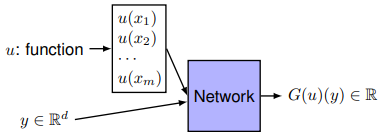
\includegraphics[width=0.5\textwidth]{img/img12.png}
    \caption{Arquitectura de las entradas necesarias para el experimento 3 propuesta en~\cite{lu2024deeponet}.}
    \label{fig:img12}
\end{figure}

Por tanto, un conjunto de entrenamiento de $n$ elementos para la subred \texttt{branch} consistirá en una matriz: 
\[
\begin{bmatrix}
u_1(x_1) & u_1(x_2) & \cdots & u_1(x_m) \\
\vdots & \vdots & \ddots & \vdots \\
u_n(x_1) & u_n(x_2) & \cdots & u_n(x_m)
\end{bmatrix}
\]

donde cada dato de entrada es un vector $[u_i(x_{1}),\dots,u_i(x_{m})]^{T}$ que representa las muestras recogidas de una función $u_{i}$, con $i=1,\dots,n$. Para este ejemplo se propociona un conjunto de entrenamiento con $n=150$ datos.

En la subred \texttt{trunk}, el conjunto de entrenamiento consiste en la partición que hemos realizado del intervalo $[0,1]$. Para este experimento se ha tomado una partición con $m=100$ elementos, lo que nos da un vector $y = [y_{1},\dots, y_{100}]$, donde cada dato de entrada corresponde al valor $y_{j}$, con $j=1,\dots,100$. 


Además, para estimar el error cuadrático de cada salida de la red se proporciona una matriz con evaluaciones explícitas del operador:

\[
\begin{bmatrix}
G(u_1)(x_1) & G(u_1)(x_2) & \cdots & G(u_1)(x_m) \\
G(u_2)(x_1) & G(u_2)(x_2) & \cdots & G(u_2)(x_m) \\
\vdots & \vdots & \ddots & \vdots \\
G(u_n)(x_1) & G(u_n)(x_2) & \cdots & G(u_n)(x_m)
\end{bmatrix}.
\] \\

\textit{SciANN} no soporta que el número de datos entrenamiento de cada subred sea distinto, es decir, requiere que $n$ sea igual a $m$. Para solucionar esto, se ha hecho una aumentación del conjunto de datos repitiendo valores y manteniendo la consistencia entre los datos de entrada y la matriz de comparaciones con la salida.

En concreto, el conjunto de datos para la subnet \texttt{trunk} es ahora un vector de 150 elemenos $y=[y_{1},\dots, y_{n=100},y_{1},\dots,y_{n-m=50}]$ y, de forma análoga, la matriz de evaluaciones de $G$ se ha extendido a

\[
\begin{bmatrix}
G(u_1)(x_1) & G(u_1)(x_2) & \cdots & G(u_1)(x_{n=100})  & G(u_1)(x_1) & \cdots & G(u_1)(x_{n-m=100}) \\
\vdots & \vdots & \ddots & \vdots \\
G(u_n)(x_1) & G(u_n)(x_2) & \cdots & G(u_n)(x_m=100) & G(u_n)(x_1) & \cdots & G(u_n)(x_{n-m=50})
\end{bmatrix}
.\] \\

Como cada fila de la matriz de salidas tiene ahora $n$ elementos, mantener la integridad entre entradas y salidas requiere modificar también el conjunto de muestras de funciones $u$ de la siguiente forma: 

\[
\begin{bmatrix}
u_1(x_1) & u_1(x_2) & \cdots & u_1(x_{m=100}) & u_1(x_1) & u_1(x_2) & \cdots & u_1(x_{n-m=50})\\
\vdots & \vdots & \ddots & \vdots \\
u_n(x_1) & u_n(x_2) & \cdots & u_n(x_{m=100}) & u_n(x_1) & u_n(x_2) & \cdots & u_n(x_{n-m=50})
\end{bmatrix}.
\]






\subsection{Construcción del modelo}\label{sec:8.4.4}

Para comprender mejor la arquitectura a implementar, nos ayudaremos de la \autoref{fig:img13} y la \autoref{fig:img15}, extraídas de~\cite{lu2024deeponet}. En ellas se puede ver cómo \textit{DeepONet} implementa dos arquitecturas inspiradas en la arquitectura dada por el \autoref{thm:p05}. Para este experimento nos ceñiremos a la la arquitectura de la \autoref{fig:img13}, que es un caso particular del teorema para $M=1$ y $N=p$.

 \begin{figure}[htbp]
    \centering
    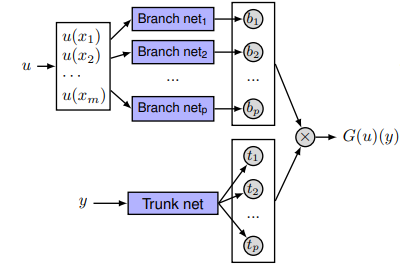
\includegraphics[width=0.4\textwidth]{img/img13.png}
    \caption{Representación compacta de la arquitectura propuesta en el \autoref{ch:sexto-capitulo} para $M=1$ y $N=p$.}
    \label{fig:img13}
\end{figure}

 \begin{figure}[htbp]
    \centering
    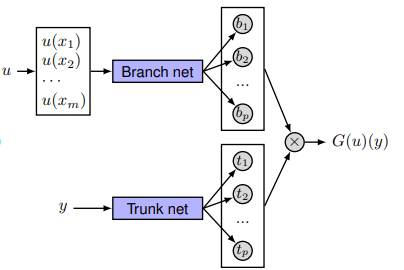
\includegraphics[width=0.4\textwidth]{img/img15.png}
    \caption{Representación compacta  de la arquitectura modificada propuesta en \textit{DeepONet}.}
    \label{fig:img15}
\end{figure}

\subsubsection{Primera aproximación}

La estructura de clases de \textit{SciANN} actualmente soporta funciones, pero no operadores. Como la arquitectura de redes neuronales en \textit{SciANN} viene ligada a funciones, es necesario cambiar a un enfoque constructivo en el que definamos exactamente las entradas y subredes neuronales que necesitamos para nuestra arquitectura, así como las relaciones entre ellas. Es por esto que se propone el modelo siguiente (\autoref{lst:exp3-aprox1}): 


\begin{lstlisting}[language=Python,caption={Primera aproximación para el modelo de aprendizaje de operadores.},label={lst:exp3-aprox1}]
#Número de sensores.
m = 100

#Número de neuronas por capa.
n_in_layer = 40

#Definicion de entradas.
x = sn.Variable("x")
ux = [sn.Variable(f'ux{i}') for i in range(m)]


#Definición de subredes.
subnet_branch = sn.Functional('branch_out', ux, [n_in_layer], activation='sigmoid')
subnet_trunk = sn.Functional("trunk_out",x ,[n_in_layer], 'sigmoid')

#Producto cartesiano de las salidas de ambas.
s  = sn.utils.dot(subnet_branch,subnet_trunk)
d1 = sn.Data(s)

#Definición del modelo.
modelo_operador = sn.SciModel(inputs = ux+[x], targets=[d1], loss_func='MSE',optimizer="adam")
\end{lstlisting}

Sin embargo, mediante el resumen del modelo y el esquema extraído por Tensorflow, que se muestra en la \autoref{fig:img14}, se puede observar que el producto escalar de la librería no está bien implementado.

 \begin{figure}[htbp]
    \centering
    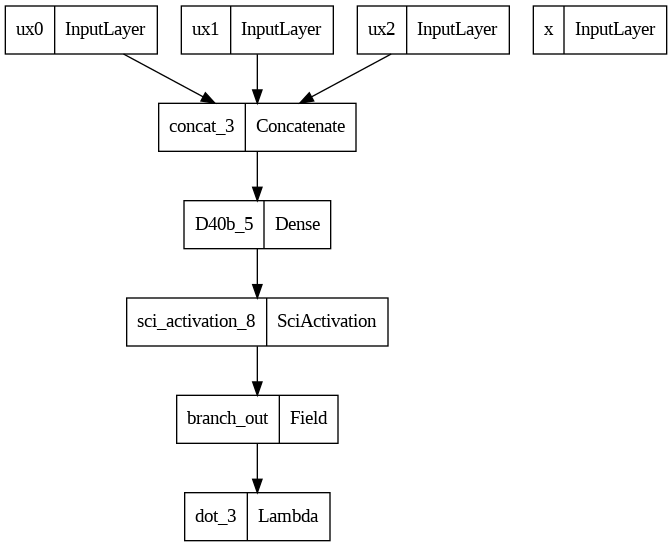
\includegraphics[width=0.5\textwidth]{img/img14.png}
    \caption{Representación interna simplificada del experimento 3: primera aproximación.}
    \label{fig:img14}
\end{figure}

\subsubsection{Segunda aproximación}\label{sec:8.4.4.2}

Debido a las dificultades encontradas, optamos por implementar el producto escalar manualmente. Recordemos que, aunque estemos definiendo las subredes como objetos de la clase \textit{Functional}, esto no va a tener ninguna repercusión en la tarea de entrenamiento, pues no hemos definido ninguna restricción que añada términos extra a la función de pérdida. 

\begin{lstlisting}[language=Python,caption={Segunda aproximación para el modelo de aprendizaje de operadores.},label={lst:exp3-aprox2}]]
#Definición de las entradas.
x = sn.Variable("x")
ux = [sn.Variable(f'ux{i}') for i in range(m)]


#Definición de subredes.

subnet_branches = [sn.Functional(f'branch_out_{i}', ux, [1], activation='tanh') for i in range(N)]
subnet_trunk = sn.Functional("trunk_out",x ,[N], 'sigmoid')

#Construcción manual del producto cartesiano de las subredes.
productos = []

for i in range(N):
  productos.append(sn.utils.mul(subnet_branches[i],subnet_trunk))

s = sn.utils.add(productos[0],productos[1])

for i in range(2,N):
  s = sn.utils.add(s,productos[i])

#Restricciones del modelo.
d1 = sn.Data(s)

#Definición del modelo.
modelo_operador= sn.SciModel(inputs = ux+[x], targets=[d1], loss_func='MSE',optimizer="adam")
\end{lstlisting}

En la \autoref{fig:operador_b} se puede observar cómo en este caso el producto entre ambas subredes se ha implementado correctamente mediante capas \textit{Lambda} de Keras. 
 \begin{figure}[htbp]
    \centering
    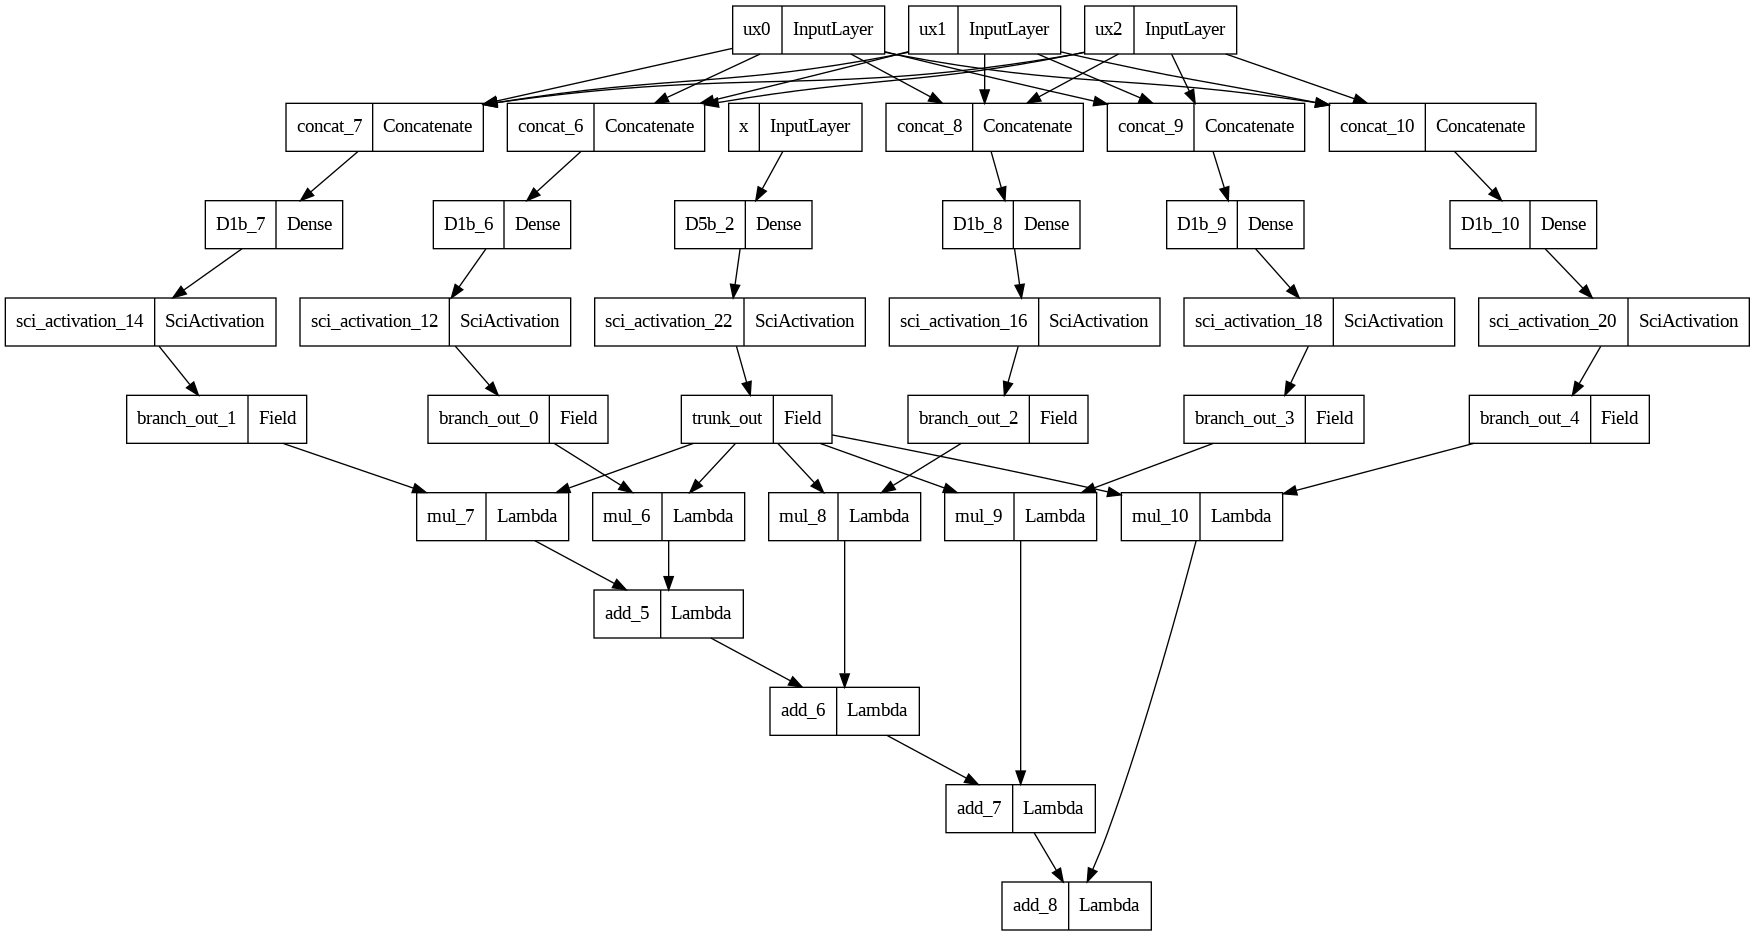
\includegraphics[width=\textwidth]{img/operador_b.png}
    \caption{Representación interna del experimento 3: segunda aproximación.}
    \label{fig:operador_b}
\end{figure}


\subsection{Interpretación de los resultados}

En esta sección vamos a comentar y comparar los resultados obtenidos para la experimentación realizada a través de la segunda aproximación al modelo. Además de realizar un ajuste de los hiperparámetros más importantes, vamos a experimentar con el tamaño de conjunto de entrenamiento. Como quedó plasmado en la \autoref{sec:8.4.3} y en la \autoref{sec:8.4.4}, ampliar el conjunto de entrenamiento requiere ampliar el número de entradas y por tanto modificar la arquitectura del modelo. Por ello, la experimentación en \textit{W\&B} se ha realizado mediante dos proyectos distintos correspondientes a los dos conjuntos de entrenamiento seleccionados. Estos proyectos pueden consultarse \hyperlink{https://wandb.ai/vaatiper-Universidad\%20de\%20Granada/projects}{aquí}.

\subsubsection{Resultados para el entrenamiento con conjunto de datos reducido}

En la \autoref{fig:img36} podemos ver cómo la experimentación no arroja mucha luz a cerca de qué hiperparámetros funcionan mejor. Al margen de alguna configuración especialmente mala, hay configuraciones muy dispares que dan resultados relativamente parecidos. Por otro lado, comparando la \autoref{fig:img36} con la \autoref{fig:img37}, se puede ver que la configuración que minimiza la pérdida en validación también minimiza la pérdida en entrenamiento. Esto es positivo, ya que indica que durante el entrenamiento no hemos sobre-ajustado el modelo al conjunto de validación. Tras ver estos resultados, se contemplan dos hipótesis. 

La primera, que no tengamos lo suficientes datos para realizar una buena tarea predictiva. La segunda hipótesis tiene que ver con que la arquitectura propuesta no sea buena para esta tarea de predicción. Ambas hipótesis pueden estar relacionadas, como explicábamos en la \autoref{sec:8.4.4.2}, con que no se hace uso de ningún tipo de restricción propia de PINNs que ayuden a la tarea de entrenamiento.  En presencia de pocos datos, dichas restricciones pueden aportar información extra que sea clave para completar satisfactoriamente la tarea de entrenamiento. 

\begin{figure}[htbp]
    \centering
    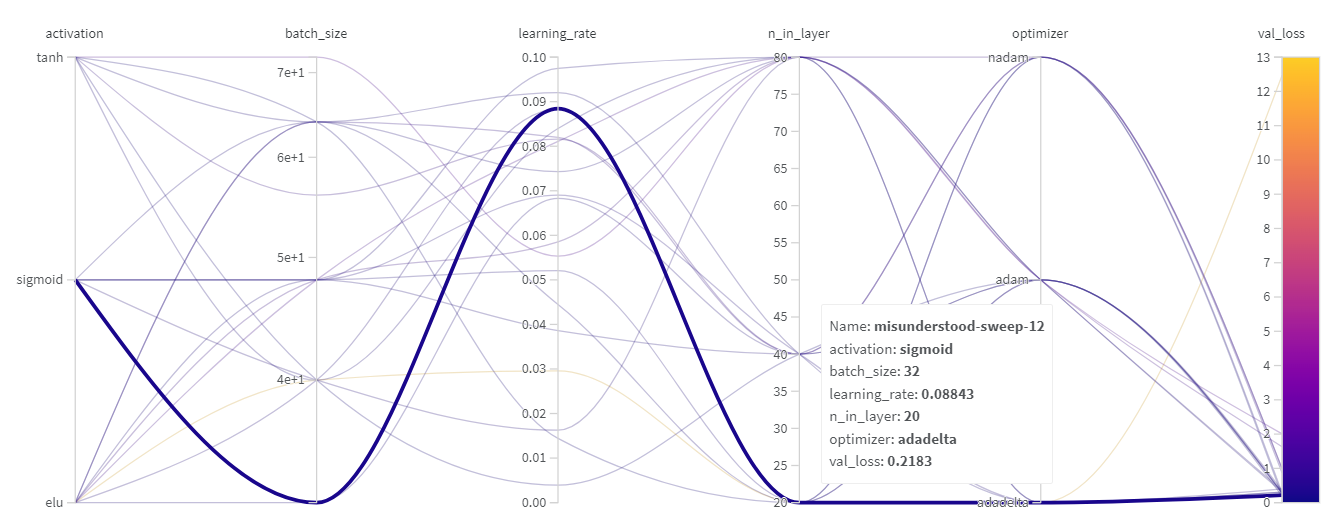
\includegraphics[width=1\textwidth]{img/img36.png}
    \caption{Desglose del ajuste de hiperparámetros para el experimento 8.3. con conjunto de datos reducido bajo la métrica \textit{val\_loss}. }
    \label{fig:img36}
\end{figure}

\begin{figure}[htbp]
    \centering
    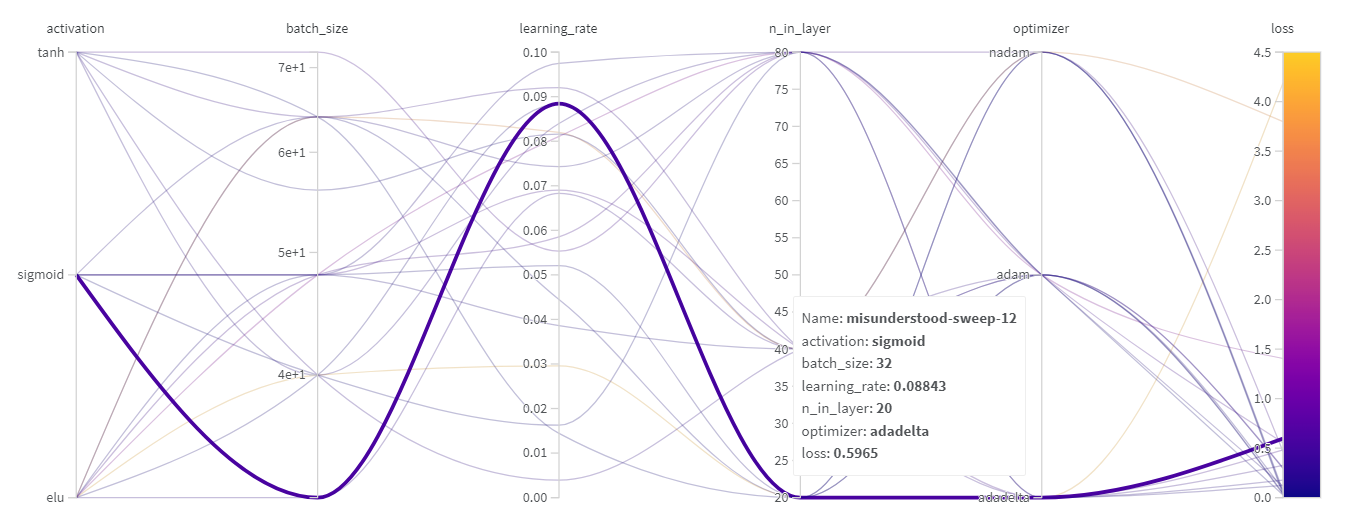
\includegraphics[width=1\textwidth]{img/img37.png}
    \caption{Desglose del ajuste de hiperparámetros para el experimento 8.3. con conjunto de datos reducido bajo la métrica \textit{loss}.}
    \label{fig:img37}
\end{figure}

\textit{W\&B} ofrece también un ranking con los parámetros que han sido más relevantes durante el proceso de entrenamiento y los que están más correlacionados con la métrica seleccionada para el entrenamiento. En la \autoref{fig:img35} podemos ver que valores altos en error están correlacionados con utilizar la función de activación ELU y el optimizador \textit{adadelta}. Sin embargo, este optimizador también está presente en la mejor configuración de parámetros encontrada. De nuevo, estos resultados apuntan a que con tan pocos datos no es posible entrenar bien el modelo. 


\begin{figure}[htbp]
    \centering
    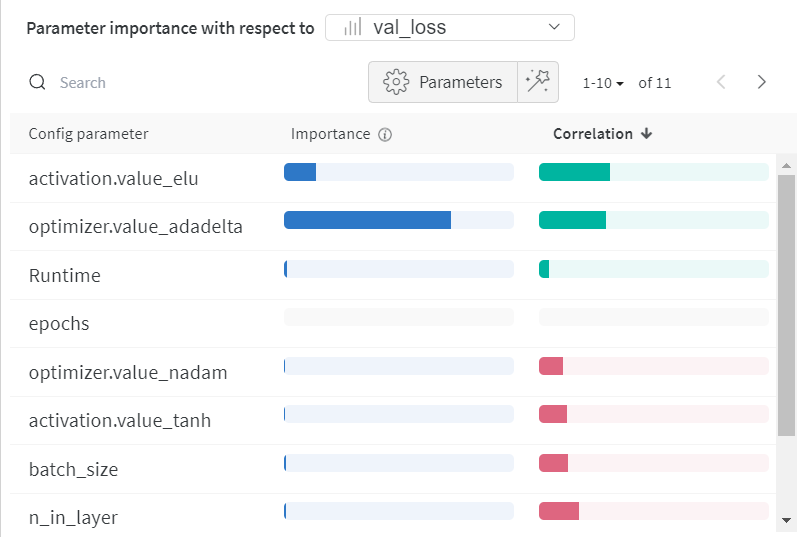
\includegraphics[width=0.6\textwidth]{img/img35.png}
    \caption{Ranking de parámetros correlacionados con la métrica \textit{val\_loss} para el experimento 8.3. con conjunto de datos reducido.}
    \label{fig:img35}
\end{figure}


Tras realizar el ajuste de hiperparámetros, se ha seleccionado el modelo que minimiza la pérdida en validación y realizado un estudio comparativo entre su evolución en entrenamiento y la evolución del modelo con la configuración de parámetros propuesta en \textit{DeepONet}, esto es, el que se corresponde con el \autoref{lst:exp3-aprox2}. El modelo que miniza la pérdida cuenta con activación sigmoidal, $20$ neuronas en la capa oculta, optimizador adadelta y un tamaño de lote de $32$ ejemplos. Aunque el entrenamiento propuesto en~\cite{lu2024deeponet} se realiza con conjunto de validación, hemos realizado también una comparativa con la evolución de entrenamiento sin utilizar conjunto de validación. Al igual que en la batería de experimentación con diferentes hiperparámetros, para el entrenamiento se ha utilizado el criterio de parada anticipada bajo las métricas de \textit{val\_loss} y \textit{loss} respectivamente.

Como podemos ver en la \autoref{fig:img6264}, el entrenamiento gobernado por \textit{val\_loss} termina muy pronto y alcanza una precisión del orden de $10^{-1}$ para \textit{val\_loss} y de $10^{-2}$ para la métrica \textit{loss}. Por otro lado, el entrenamiento sin conjunto de validación alcanza valores de pérdida del orden de $10^{-4}$ cercanos a las precisiones alcanzadas por la implementación en \textit{DeepONet}. Sin embargo, en ambos casos, al realizar la predicción sobre el conjunto de test la precisión no baja de $10^{-1}$. 



\begin{figure}[htbp]
    \centering
    \begin{subfigure}{0.45\textwidth}
    \centering
    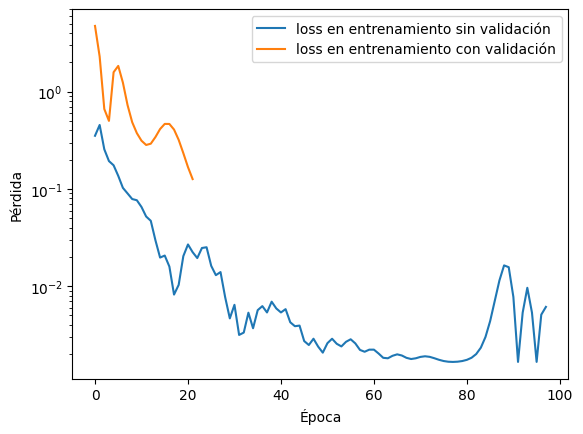
\includegraphics[width=\linewidth]{img/img62.png} 
    \caption{Modelo propuesto en \textit{DeepONet}.}
    \label{fig:img62}
    \end{subfigure}   
    \begin{subfigure}{0.45\textwidth}
    \centering
    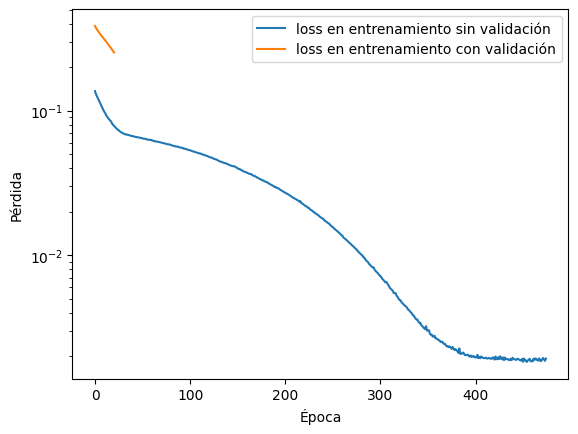
\includegraphics[width=\linewidth]{img/img64.png}
    \caption{Modelo seleccionado.}
    \label{fig:img64}
    \end{subfigure}
\caption{Comparación entre los modelos seleccionados para el conjunto de entrenamiento reducido.}
\label{fig:img6264}
\end{figure}

\subsubsection{Resultados para el entrenamiento con conjunto de datos ampliado}

En el diagrama de la \autoref{fig:img40} se muestran los detalles de la experimentación realizada con todos los datos de entrenamiento disponibles, adaptando la arquitectura del modelo para ello. Como se puede ver en una comparación con la \autoref{fig:img41}, aunque la pérdida en validación se mantenga en el orden de $10^{-1}$, la pérdida en entrenamiento sí disminuye. Una vez más, el modelo se sobre-ajusta a los datos de entrenamiento, cuya precisión difiere significativamente de la obtenida en validación. De estos resultados deducimos que las limitaciones para la predicción se deben a la arquitectura y proceso de entrenamiento del modelo, ya que para los mismos conjuntos de datos el modelo de~\cite{lu2024deeponet} realiza predicciones en validación con precisiones del orden de $10^{-4}$. 

\begin{figure}[htbp]
    \centering
    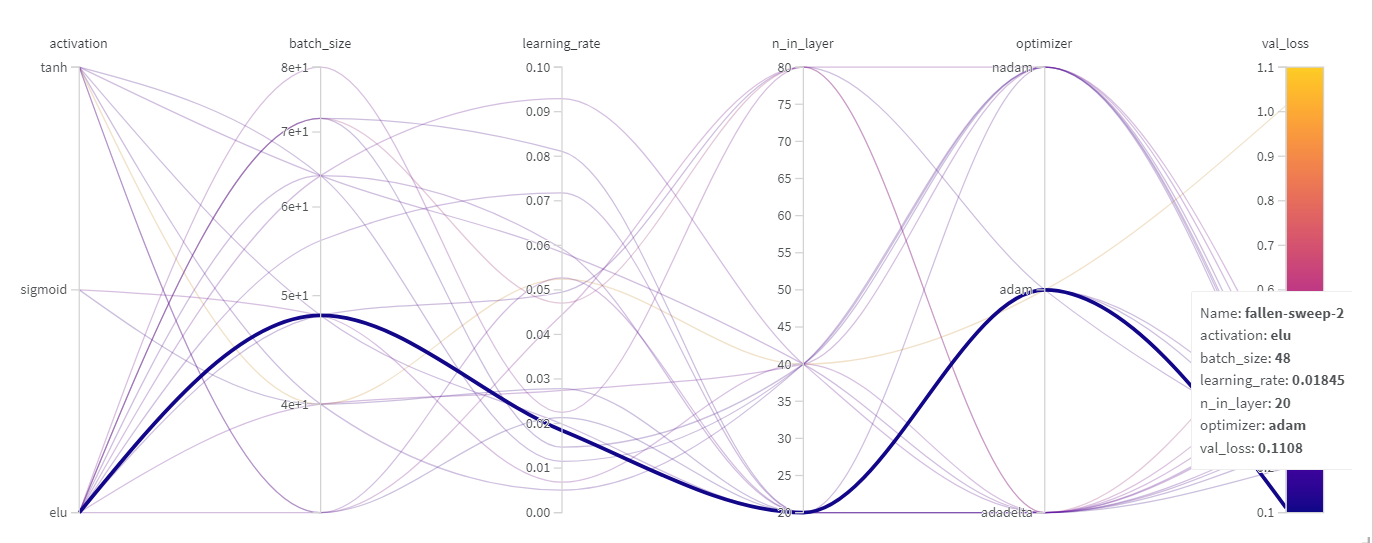
\includegraphics[width=1\textwidth]{img/img40.png}
    \caption{Desglose del ajuste de hiperparámetros para el experimento 8.3. con conjunto de datos ampliado bajo la métrica val\_loss. }
    \label{fig:img40}
\end{figure}

\begin{figure}[htbp]
    \centering
    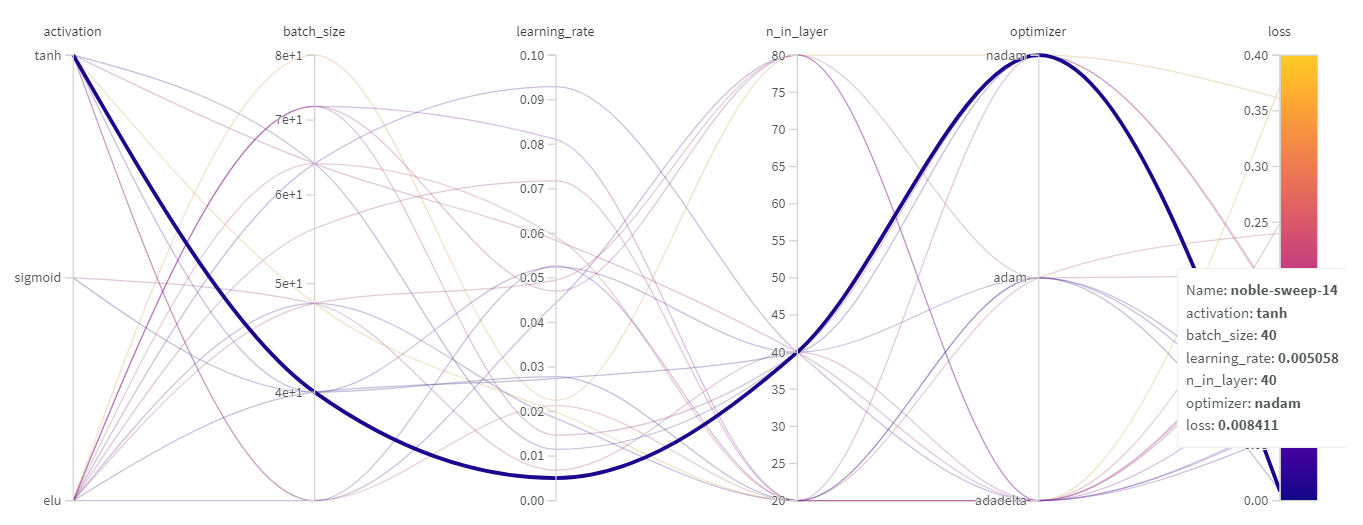
\includegraphics[width=1\textwidth]{img/img41.png}
    \caption{Desglose del ajuste de hiperparámetros para el experimento 8.3. con conjunto de datos ampliado bajo la métrica loss.}
    \label{fig:img41}
\end{figure}

 Aunque no hayamos conseguido mejoras significativas en la tarea de aprendizaje, el ranking mostrado en la \autoref{fig:img39} parece dar información más coherente sobre el modelo que el ranking del apartado anterior. El parámetro de configuración más correlacionado con valores altos en \textit{val\_loss} es la anchura de la capa profunda, \textit{n\_in\_layer}. Volviendo a la \autoref{fig:img40}, podemos corroborar que la mayoría de combinaciones que partían de un valor elevado para este parámetro han resultado en errores de validación grandes.  Para justificar esto, es necesario recordar que la predicción no es buena en validación pero sí en entrenamiento. Esto indica un sobre-ajuste a los datos de entrenamiento. Este escenario puede deberse a trabajar con modelos complejos, con demasiados grados de libertad, como es el caso de nuestro modelo cuando \textit{n\_in\_layer} toma valores grandes. La aproximación del operador es mejor para modelos más simples y, por tanto, no es que nuestra tarea sea demasiado compleja para el modelo, si no que la arquitectura y proceso de entrenamiento no se adecuan bien al aprendizaje.




\begin{figure}[htbp]
    \centering
    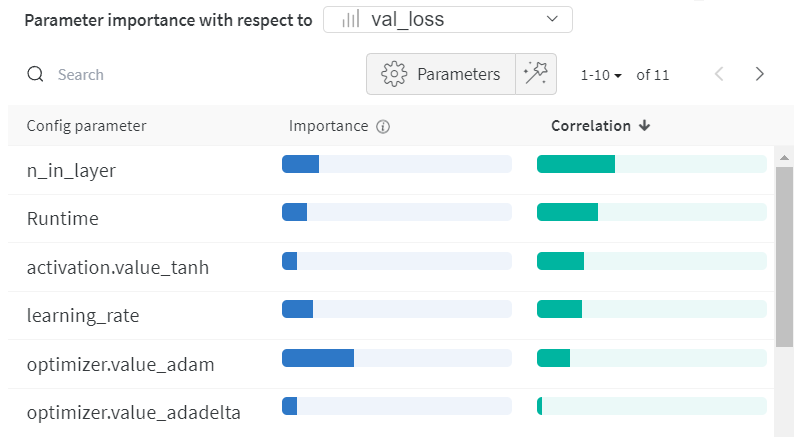
\includegraphics[width=0.6\textwidth]{img/img39.png}
    \caption{Ranking de parámetros correlacionados con la métrica val\_loss para el experimento 8.3. con conjunto de datos ampliado.}
    \label{fig:img39}
\end{figure}

Por último, volvemos a realizar una comparación entre los entrenamientos del mejor modelo encontrado durante la experimentación y el modelo propuesto en el \autoref{lst:exp3-aprox2}. Como podemos ver en la \autoref{fig:img6365}, la evolución es muy similar a la que obteníamos en el apartado anterior. Aunque para ambos modelos se ha conseguido más precisión en el conjunto de entrenamiento, recordemos que la precisión en los conjuntos de validación y test se mantiene en el orden de $10^{-1}$, por lo que consideramos que ampliar el conjunto de entrenamiento no ha mejorado la tarea de aprendizaje. 

\begin{figure}[htbp]
    \centering
    \begin{subfigure}{0.45\textwidth}
    \centering
    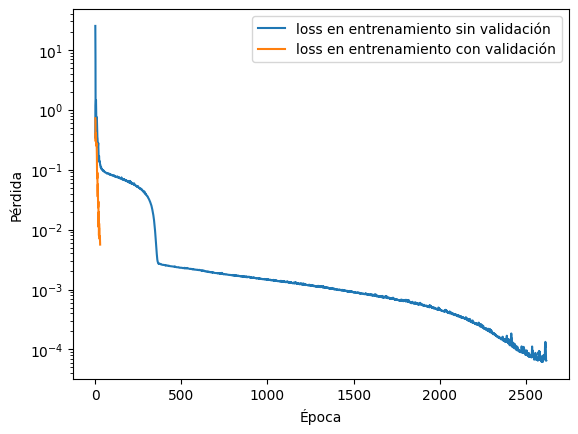
\includegraphics[width=\linewidth]{img/img63.png} 
    \caption{Modelo propuesto en \textit{DeepONet}.}
    \label{fig:img63}
    \end{subfigure}   
    \begin{subfigure}{0.45\textwidth}
    \centering
    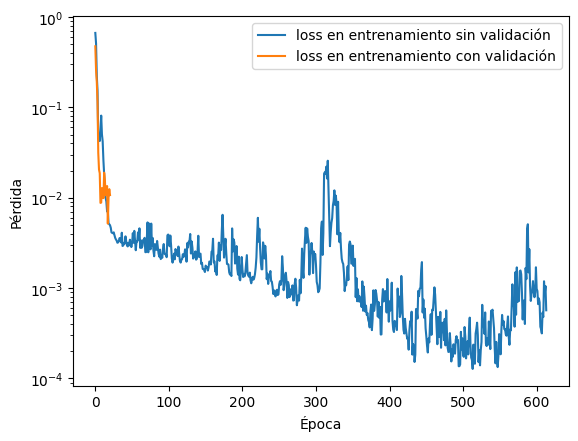
\includegraphics[width=\linewidth]{img/img65.png}
    \caption{Modelo escogido tras experimentación.}
    \label{fig:img65}
    \end{subfigure}
\caption{Comparación entre los modelos seleccionados para el conjunto de entrenamiento ampliado.}
\label{fig:img6365}
\end{figure}

\subsubsection{Interpretación}

Tras las experimentaciones realizadas, hemos visto que los modelos pueden llegar a ajustarse a los datos de entrenamiento proporcionados pero, sin embargo, no generalizan bien. La poca capacidad de generalización se mantiene incluso para los modelos más simples, lo que descarta un sobre-ajuste a los datos de entrenamiento debido a la complejidad del modelo. Este hecho, junto con los buenos resultados obtenidos en~\cite{lu2024deeponet} para el mismo conjunto de datos, demuestra que la incapacidad para aproximar operadores no recae sobre el conjunto de datos seleccionado, si no sobre las abstracciones, arquitectura y proceso de entrenamiento que a día de hoy \textit{SciANN} soporta para esta tarea. Con todo esto, se concluye que ninguno de los modelos ha sido capaz de realizar la tarea de aprender operadores globalmente. Esto se atribuye principalmente a la incapacidad de \textit{SciANN} para integrar el aprendizaje de operadores desde el enfoque de las PINNs. 